\documentclass[english]{DESCARWINreport}

\usepackage{times}
\usepackage{helvet}
\usepackage{courier}
\usepackage{graphicx}
\usepackage{multirow}
%\usepackage[utf8]{inputenc}
\usepackage{algorithm}
\usepackage[noend]{algorithmic}
\usepackage{amsmath}
\usepackage{amsfonts}
\usepackage{amssymb}
\usepackage{array}
\usepackage{subfigure}
\usepackage{lscape}
%\usepackage{aaai}

\algsetup{indent=1.8em}
\renewcommand{\algorithmiccomment}[1]{// #1}
\newcommand{\pp}{planning tasks}
\newcommand{\PP}{planning task}
\newcommand{\dae}{{\em Divide-and-Evolve}}
\newcommand{\DAEI}{{\sc D\&E}}
\newcommand{\DAEII}{{\sc DaE2}}
\newcommand{\DAE}{{\sc DaE}}
\newcommand{\DAEX}{{\sc DaE$_{\text{X}}$}}
\newcommand{\DAEYAHSP}{{\sc DaE$_{\text{YAHSP}}$}}
\newcommand{\CPT}{{\sc CPT}}
\newcommand{\LPG}{{\sc LPG}}
\newcommand{\LAMA}{{\sc LAMA}}
\newcommand{\TFD}{{\sc TFD}}
\newcommand{\YAHSP}{{\sc YAHSP}}
\newcommand{\OPENSTACKS}{{\sc Openstacks}}
\newcommand{\ELEVATORS}{{\sc Elevators}}
\newcommand{\CREWPLANNING}{{\sc CrewPlanning}}
\newcommand{\FLOORTILE}{{\sc Floortile}}
\newcommand{\PARCPRINTER}{{\sc ParcPrinter}}
\newcommand{\bm}{{b_{max}}}


\def\UU{{\mathbb{U}}}

%\title{DESCARWIN\\\bigskip {\em \LARGE The Marriage of Descartes and Darwin}\\\bigskip \bigskip \bigskip \bigskip \bigskip \bigskip \bigskip {\LARGE WP1: the \DAEX\ Planning System}}
\title{DESCARWIN\\\bigskip {\em \LARGE The Marriage of Descartes and Darwin}\\\vspace{8cm} {\LARGE D5.4: Inoculation}}
%ANR-09-COSI-002
%\author{Yann Semet}
\date{\today}
\laboratory{TRT - INRIA - ONERA}
\docref{62 441 217-179-6}

\revision{-}

%\setlength{\parindent}{0cm}
%\setlength{\parskip}{2ex plus 0.5ex minus 0.2ex}


% Pour réduire globalement l'espace entre les items d'une liste
% on peut également utiliser le bout de code suivant de M. Wooding
% Les paramètres utilisés pour définir cette mise en page
% sont les suivants :
% \topsep espace vertical supplémentaire (ajoute à \parskip)
% 	inséré entre le texte précédant la liste et le 1er objet
% 	de la liste
% \partosep espace vertical supplémentaire inséré devant la liste
% 	si celle-ci est précédée d'une ligne blanche
% \itemsep espace vertical supplémentaire (ajouté à \parsep)
% 	inséré entre les éléments d'une liste.

%%%% debut macro %%%%
\makeatletter
\toks@\expandafter{\@listI}
\edef\@listI{\the\toks@\setlength{\parsep}{0pt}}
\edef\@listI{\the\toks@\setlength{\topsep}{0pt}}
\makeatother
%%%% fin macro %%%%


\begin{document}

\maketitle

%\cleardoublepage

\begin{revisions}
\begin{revtable}
\dates{May 31, 2013}{}{}{}
\writers{Yann Semet\\Pierre Sav\'eant}{}{}{}
\approvers{P. Sav\'eant}{}{}{}
\end{revtable}
\begin{revisionlabels}
\revlabel{initial version}
\revlabel{}
\end{revisionlabels}
\end{revisions}

\begin{abstract}
This document provides the description and experimentation of work conducted to improve the initialization phase of the \DAE's evolutionary engine. We focus, in particular, on initialization procedures built around an individual provided either by specific construction or by invoking external planners. Following the biological metaphor inherent to evolutionary algorithms, such procedures are usually called ``artificial insemination'' or ``inoculation'' in the literature, we choose to stick to the latter. Two experimental campaigns are reported here. 

The first one is our early attempt at designing an inoculation procedure that builds the initial population around an individual constructed by our embedded planner, \YAHSP, with an additional routine designed to produce a consequently refined estimate of the critical parameter defining \YAHSP's exploratory allowance once the search has started, {$b_{max}$}. Experimental results show very poor performance and high risk of runs, with ``unlucky'' random seeds, getting stuck in fruitless sampling of the search space. 

The second set of experiments follows a different strategy, getting rid of \YAHSP\ as the inoculant provider on one hand and being far more parsimonious with {$b_{max}$} on the other hand. We use additional sampling both to compensate for {$b_{max}$}'s restricted increase and to produce the inoculant. We call this procedure ``Inoculation through mass selection''. Experimental results exhibit both substantial improvements in speed and risk reduction for our algorithm, albeit on a limited subset of the entire IPC benchmark. 

\end{abstract}

\tableofcontents

\newpage

\chapter{Introduction}

\begin{quotation}
\emph{``It is difficult to catch a black cat in a dark room, especially when it is not there.''}
\begin{flushright}
Chinese Proverb

\end{flushright}
\end{quotation}

\vspace{0cm}

\section{Context}

Search is about finding things that are difficult to locate. Stochastic search, evolutionary or otherwise, is about injecting randomness in the process when the field is so large or labyrinthine one has no other choice anyway. The challenge however, like the devil, is in the details of that randomness. There are many things one can do to improve one's odds of finding what one is looking for: throwing more light in, work in teams, use binoculars, ask someone, run faster, search deeper and so forth. All of these tricks have counterparts in mathematical optimization and computational search: local sampling, parallel search, depth first search, external expert knowledge, relaxed constraints, hybrid algorithms, etc. It all boils down to injecting whatever form of intelligence, knowledge or power is available at reasonable cost in the stochastic process to tame and steer randomness in the right direction.

Evolutionary algorithms offer many such avenues of improvement. They are usually made of many interconnected heuristically designed modules, each of which performing some portion of the traditional genetic loop with some flavor of randomness: initialization, selection, reproduction, blind variations, replacement, stopping criteria. Representation, helper or hybridized algorithms and genotype mappings can also benefit from efforts to build an intelligent bias for random search. \DAE\ makes no exception: it is an evolutionary algorithm coupled with an embedded AI planner. It has a convoluted workflow, five variation operators and dozens of parameters and routines, many of which have been designed or tuned with somewhat arbitrary randomness based ingredients which can be improved with externally provided intelligence.

In that perspective, the traditional evolutionary building block the present report deals with is \emph{initialization}. More specifically, we look at how the initial population, and therefore the entire algorithm, can be improved by being made less pointlessly random from the start. The idea is to find a way to start the search directly from an interesting zone instead of blindly sampling the search space as is usually done by default. One possible way to do this is known as \emph{inoculation}. In biology or medicine, inoculation refers to ``the placement of something that will grow or reproduce, and is most commonly used in respect of the introduction of a serum, vaccine, or antigenic substance into the body of a human or animal, especially to produce or boost immunity to a specific disease''. In our mathematical context we will seek to find a way to quickly construct one individual with a good fitness value or good building blocks and use variations of that individual to constitute the initial population. That individual, which we will call the \emph{inoculant} will serve as the vehicle for the injection of interesting search space information into the genetic population where it will be spread and sampled along with successive generations.  Obviously enough, this process relies on the assumption that we can design a way to fabricate this individual both quickly enough and with enough interesting material for inoculation to be worth the extra cost in algorithmic terms.

To sum up, and come back to our metaphoric epigraph, we will henceforth try to catch the cat faster by starting at least from the right room.

\section{State of the Art: The Seven Motivations of Highly Effective Inoculations}


As mentioned earlier, the main rationale behind inoculation is to steer randomness in the right direction by injecting external knowledge into your population. There are several such forms of knowledge and just as many potential benefits to motivate you to try to improve your algorithm with an inoculation procedure:

\begin{description}

\item[Motivation 1 : Bypassing ``Senseless Randomness''] 

Optimization fitness plots are usually very steep over early iterations or generations. It usually means that vast portions of the search space can be quickly discarded as being senseless for the problem at hand where interesting things only happen within the bounds of a restricted set of parameter intervals. A reasonable approximation of these intervals can usually be obtained quickly, either by design, heuristics or sampling, and inoculation, based on that estimate can serve the purpose of ``starting directly from the bottom of the curve'' which can represent a usually small but sometimes substantial fraction of the total run time. Another example where large savings can be obtained by cutting through trivial search has to do with order based approaches, such as permutation based algorithms typical of combinatorial optimization, where early generations are usually spent running for a first reasonable permutation which makes sense with respect to problem data. The \emph{h1} heuristic used by \DAE\ is an example of substantial improvement obtained in this manner: it prevents the consideration of decompositions which do not make sense in terms of earliest possible start dates for atoms.

\item[Motivation 2 : Taking Time to Precompute]

An optimization problem is usually made of both generic domain information and specific settings for the problem at hand. Both contain many items that can be useful when solving the actual problem, i.e. when the search has started. These items can be secured through precomputations and later fed to the search algorithm, for instance by inoculation in the initial population. These precomputations can indeed often be modeled as partial solutions and be used to construct individuals. An example in AI planning is \emph{landmarks}, which are facts that ``must be true at some point on any solution path to the given planning task.'' \cite{DBLP:journals/corr/abs-1107-0052}. Knowing such facts before starting the search can help restrict it to a smaller number of reasonable paths.

\item[Motivation 3 : Solving a Relaxed Version of the Problem]

One fundamental technique in Operations Research and Mathematical Programming is to consider a relaxed version of the problem one is about to solve. Relaxed means without taking some or all constraints into account. Solutions to the relaxed problem and solutions to the actual problem often share many characteristics and the relaxed version, which can usually be obtained way more easily and quickly can be an excellent informant. It can, for instance, serve as the basis for an admissible heuristic providing a lower bound on the best possible solution in terms of the objective function, which can be used to guide the \emph{A*} algorithm in its search of a solution path. An inoculant based on a relaxed solution could be an excellent way to quickly identify elementary characteristics common to all good solutions. 


\item[Motivation 4 : Having a First Shot at the Actual Problem]

In a spirit similar to the previous motivation concerning relaxed solutions, if you have access to an external solver that is able to very quickly find a viable solution to your full problem, albeit with poor fitness performance, or if you can tune your solver to do that, you may have an excellent way to jumpstart your search! The creation of the inoculant in this case is moreover straightforward because what you obtain is already a complete, viable solution or individual.

\item[Motivation 5 : Algorithm portfolios]

Extending over motivation 4, if you have several solvers with varying performance characteristics, the best possible strategy might be to combine their respective strengths with a hybrid scheme, possibly based on conditions identifying the best one use in a given context. Inoculation can act as one such strategy in several ways, as it can: 1) hybridize a fast but suboptimal solver with a deep solving one by giving a small initial time slot to the former and leaving the rest to the latter 2) hybridize metric sensitive solvers or solvers with abilities pertaining to different aspects of the solutions with similar time allowances in a relay race inspired fashion 3) allow many different solvers to offer a variety of inoculated starting points to be genetically mixed.

\item[Motivation 6 : Solution Portfolios and Domain Experts]

Real-World optimization efforts could not be successful without domain experts. Algorithms, sophisticated as they might be, can only be efficient if they manipulate the right data in the right way and applying out-of-the-box algorithms on raw field data is bound to lead nowhere in the vast majority of cases. Any optimization campaign should be based on a dialogue between the computer scientist and the domain expert, the former incorporating information provided by the latter into the various parts of her algorithms and data structures. One thing experts often provide is solution patterns or portfolios: ``in context XYZ, ABC is a good plan''. These patterns often can be seen as partial solutions and can be inoculated if one can come up with a way of constructing full individuals with these building blocks. An example of ``primordial soup'' of good building blocks serving as the basis for the initial population can be seen in Messy Genetic Algorithms \cite{Kargupta95search}.

\item[Motivation 7 : Statistics and Sampling]

One thing one might want to attempt before launching the actual search is to use purely random sampling to get a quick idea of the shape of the search space with respect to the degrees of freedom at hand, an idea generalized by Estimation of Distribution Algorithms \cite{Baluja95removingthe, Larranaga:2002b}
. There is always a compromise to be found in stochastic search between keeping on sampling and moving on to other parts of the search space and this compromise is usually particularly sensitive at the beginning of the search, especially with fast or prematurely converging algorithms. You may therefore want, in fear of local optima, to inoculate your initial population with strong individuals identified through fast but extensive preliminary surveys.


\end{description}

%\newline
%\newline

In spite of these numerous possible motivations, there are at least two potential drawbacks to inoculation that the designer will want to keep in mind. The first one takes place within the traditional quest evolutionary computation practitioners are all familiar with: the infamous exploration/exploitation tradeoff. If helping the search by having it start from an interesting zone can obviously speed things up, it can also turn out be an insidious bias leading to a local optimum and therefore be a source of premature convergence. Several countermeasures can be imagined: use several inoculants coming from different external sources, build an initial population filling routine with a carefully crafted use of variations to ensure sufficient variety, having a mixed scheme with both inoculants and purely random individuals and so on. The second drawback is that inoculation procedures are, most of the time, highly problem specific and therefore force you to make a step away from the admittedly utopian dream of a generic solver.

Extensive discussion of inoculation to boost evolutionary search can be found in \cite{Surry96, SurryPhD}. An example of inoculation in a real-world context with substantial benefits can be found in \cite{semetGECCO06} where the technique is used to solve a railroad based combinatorial problem faster by using aforementioned motivations 1, 2 and 3.


%\section{State of the Art}
%Messy GAs \cite{Kargupta95search}, PBIL \cite{Baluja95removingthe}, EDAs \cite{Larranaga:2002b}
%Surry \cite{Surry96, SurryPhD}
%Semet \cite{semetGECCO06}


\newpage
\chapter{Inoculation with YAHSP}

In this section, we describe and motivate the actual basic inoculation procedure we designed in the first place and present experimental results that show its inefficiency in several respects. We then introduce, also along with experiments, another way to boost our evolutionary initialization phase which brings improvements with respect to both stochastic risk and computation speed. We call this procedure Inoculation through Mass Selection (IMS).

\section{Formalizing inoculation procedures}

To make things more explicit, an inoculation procedure is made of the following components:

\begin{description}

\item[A substance provider] 

This module is responsible for providing the substance to be injected in the population. It is usually a separate, externally provided module that is able to produce an individual or part of it.

\item[An inoculant builder] 

In case the provided substance is not a complete individual, a procedure is necessary to construct an full individual around it and insert it in the population. This individual is called the inoculant.

\item[A variation scheme] 

To ensure sufficient diversity for the genetic search to be exploratory enough, variations must be applied to the inoculant to produce variants in order to fill the population.


\item[A composition scheme] 

The initial population will be filled with inoculant variants but to an extent that can be defined by the algorithm designer. More elaborated schemes can also be imagined where several substance providers are put to work. The composition scheme will detail how the initial population will be composed between purely random individuals and the substance enriched inoculants provided by various sources.


\end{description}

\section{Meet Adam!}

The initialization/inoculation procedure works as follows and as outlined by algorithms 1 through 4. Algorithm 1 gives the global outline of our initialization, which work in two separate phases: the initial population is first built by gathering randomly generated individuals and then, an estimation for {$b_{max}$}, a critical parameter setting the embedded planner's exploratory allowance, is computed by manipulating the population. As outlined in algorithm 2 described in more depth elsewhere \cite{DBLP:conf/aips/BibaiSSV10}, the random generation procedure follows an intermediate goal setting heuristic framed by a minimal timestamp computing heuristic, {$h1$}, and randomly fills the individuals' predefined goals with random atoms picked while respecting mutex constraints. In the normal case, without inoculation, algorithm 3 proceeds to estimate the proper value for {$b_{max}$} in an incremental manner: its value is increased until a sufficient number of feasible individuals is present int the population as an individual, i.e. a decomposition of the planning problem in intermediate goals, can be declared feasible or not depending on how extensively \YAHSP\ is allowed to work on it, which is determined by {$b_{max}$}.

\begin{algorithm}[h!]
\caption{Initialization}
\label{algoInit}
{\small
\begin{algorithmic}[1]
\REQUIRE{$N, b_{max}\-fixed, b_{max}\-ratio, b_{max}\-lastweight, b_{max}\-increase, insemination$} \hfill \COMMENT{initialization parameters}

\FOR{$i \in [1..N] $}
\STATE{$pop[i] \leftarrow GenerateIndividual(K)$} \hfill \COMMENT{random individuals with K intermediate goals}
\ENDFOR

\IF{$(b_{max}\-fixed \ne 0)$} 
\STATE{$b_{max} = b_{max}\-fixed$}
\ELSE
\IF{$(insemination==1)$}
\STATE{$b_{max} = estimate b_{max} insemination(b_{max}\-ratio,b_{max}\-increase)$}
\ELSE
\STATE{$b_{max} = estimate b_{max} incremental(b_{max}\-ratio,b_{max}\-increase)$}
\ENDIF 
\ENDIF
\STATE{$b_{max}last = b_{max} * b_{max}\-lastweight$}
\end{algorithmic}
}
\end{algorithm}

\begin{algorithm}[h!]
\caption{generateIndividual(N)}
\label{algoGenerate}
{\small
\begin{algorithmic}[1]
\REQUIRE{$T$} \hfill \COMMENT{candidate start times}
\STATE{$D \leftarrow \{\}$}\hfill \COMMENT{ordered list of timestamps}
\REPEAT
\STATE{$t \leftarrow \UU(T)$} 
\STATE{$T \leftarrow T \setminus \{t\}$} 
\STATE{Insert($t,D)$} \hfill  \COMMENT{maintain $D$ ordered}
\UNTIL{$\#D = N$}
\STATE{$\text{Ind} \leftarrow \{\}$}  \hfill \COMMENT{start building the individual}
\FOR{$t \in \ D $}
\STATE{$s \leftarrow \{\}$} \hfill \COMMENT{start building the intermediate goal}
\STATE{$A_t \leftarrow \{a \in A\;|\;T(a) = t\}$}    \hfill \COMMENT{atoms that can appear at $t$}
\STATE{$n \leftarrow \UU([1,\#A_t])$} \hfill \COMMENT{number of atoms} \label{init.state}
\WHILE{$n \neq 0 \wedge A_t \neq \{\}$} \label{begin.loopInit}
\STATE{$a \leftarrow \UU(A_t)$}    \hfill \COMMENT{choose uniformly an atom in $A_t$}
\STATE{$s \leftarrow s \cup \{a\}$}   \hfill \COMMENT{add to $s$}
\STATE{$A_t \leftarrow A_t\setminus \left(\{a\} \cup M(a)\right)$ }  \hfill \COMMENT{remove all mutex}
\STATE{$n \leftarrow n-1$}
\ENDWHILE \label{end.loopInit}
\STATE{$\text{Ind} \leftarrow \text{Ind} + \{s\}$}  \hfill \COMMENT{add the new intermediate goal}
\ENDFOR
\RETURN{Ind}
\end{algorithmic}
}
\end{algorithm}

The inoculation procedure is an alternative to the aforementioned incremental {$b_{max}$} estimation procedure. It is detailed in algorithm 4. It works in several steps. First, it calls \YAHSP\ for a quick solution on the entire planning problem. Then, this solution plan is converted to a decomposition with intermediate goals to make up an individual ready for genetic mixing. This new individual will serve as the \emph{inoculant}, we call it \emph{Adam} for reference purposes. The initial population is then reconstructed using identical copies of \emph{Adam}. A double loop routine follows, both to introduce diversity and to produce a relevant estimate for {$b_{max}$}. Following a classical constraint handling technique, we try to push the population towards the infeasibility border. To do so, \emph{delgoal} mutations are first applied to all individuals iteratively until a sufficient number of them are pushed to infeasibility. Then {$b_{max}$} is iteratively increased until the population reaches the specified ratio of feasible individuals back. Having done all that, the population is made of borderline feasible variants of Adam, a supposedly stronger than random individual, and {$b_{max}$} is set to a proper value. The search can start...

So in terms of our formalism:

\begin{center}
\begin{tabular}{|l|l|}
  \hline
  \multicolumn{2}{|c|}{\bf Basic Inoculation} \\
  \hline
  \emph{Substance provider} & YAHSP \\
  \emph{Inoculant builder} & 1 to 1 decomposition \\
	\emph{Variation scheme} & \emph{delgoal} mutations to infeasibilty \\
	\emph{Composition scheme} & All inoculant variants \\
  \hline
\end{tabular}
\end{center}

\begin{algorithm}[h!]
\caption{$estimate b_{max} incremental$}
{\small
\begin{algorithmic}[1]
\REQUIRE{$N, b_{max}\-fixed, b_{max}\-ratio, b_{max}\-lastweight, b_{max}\-increase, b_{max}\-max, insemination$}

\STATE{$b_{max} \leftarrow 1$}
\STATE{$goodguys \leftarrow 0$}
\STATE{$goodguysMin \leftarrow N * b_{max}\-ratio$}
\WHILE{$( (goodguys < goodguysMin) AND (b_{max} < b_{max}\-max) )$}
\FOR{$i \in [1..N] $}

\IF{$pop[i].isFeasible()$}
\STATE{$goodguys++$}
\ENDIF
\ENDFOR
\STATE{$b_{max} *= b_{max}\-increase$}
\ENDWHILE

\RETURN{$b_{max}$}
\end{algorithmic}
}
\end{algorithm}

\begin{algorithm}[h!]
\caption{$estimate b_{max} insemination$}
{\small
\begin{algorithmic}[1]
\REQUIRE{$N, b_{max}\-fixed, b_{max}\-ratio, b_{max}\-lastweight, b_{max}\-increase, b_{max}\-max, insemination$}

\STATE{$solutionPlan \leftarrow yahspCreateAdam()$}
\STATE{$Adam \leftarrow convertToDecomposition(solutionPlan)$}
\STATE{$eval(Adam)$}
\FOR{$i \in [1..N] $}
\STATE{$pop[i] \leftarrow Adam$}
\ENDFOR

\STATE{$goodguys \leftarrow 0$}
\STATE{$goodguysMin \leftarrow N * b_{max}\-ratio$}

\WHILE{$(goodguys > goodguysMin)$}
\STATE{$goodguys \leftarrow 0$}
\FOR{$i \in [1..N] $}
\STATE{$mutate(pop[i])$}
\STATE{$eval(pop[i])$}
\IF{$pop[i].isFeasible()$}
\STATE{$goodguys++$}
\ENDIF
\ENDFOR

\ENDWHILE
\WHILE{$((goodguys < goodguysMin)AND(b_{max}<=b_{max}\-max))$}
\STATE{$eval(pop)$}
\STATE{$b_{max} *= b_{max}\-increase$}
\ENDWHILE

\RETURN{$b_{max}$}
\end{algorithmic}
}
\end{algorithm}


\newpage

\section{Experiments}

To evaluate the performance of our inoculation procedure, we conducted a number of experiments over several instances of several domains of the 7th International Planning Competition (IPC7). The bottom line of these experiments is that as such, our inoculation procedure performs very poorly compared to the normal initialization procedure. We report here a few significant experiments.

In all cases, we use \dae's default parameters : a population size of 100, a deterministic tournament of size 5, 700 offsprings, a goal neighborhood radius of 2, changeAtom and delAtom mutations both with 0.8 probabilities (per atom), a crossover probability of 0.2, mutation probability of 0.8 and weights for delgoal, addgoal, delatom, addatom of 1,3,1 and 1 respectively. We use a bmax ratio of feasibility of 1\%, a bmaxlastweight of 3 and a bmaxincreasecoeff of 2.

For the first set of experiments, we launch \dae\ with and without basic inoculation and center our observations on two parameters: the average fitness value for Adam as opposed to the average fitness value of the best individual in a random population on one hand and the average speed at which the individuals can be processed, which we measure as the average time it takes to reach the first generation. All results are averaged over several seeds.

As can be seen in figures \ref{fig:adam_el}, results are consistent over all test domains, here \ELEVATORS, \OPENSTACKS\ and \FLOORTILE\ and over all instances, of increasing difficulty: Adam has a very poor fitness value, as exemplified by the \ELEVATORS\ P01 case where it starts around 4000 where the average random population starts around 2000. Fitness values are less contrasted with \OPENSTACKS\ but still give the same picture as do the \FLOORTILE\ results. In terms of speed, the qualitative conclusion is the same and even more spectacularly so, except for \FLOORTILE: inoculating Adam results in a considerably slower, up to a factor of 10, algorithm than proceeding with randomly generated individuals. Preliminary analysis suggest that Adam's poor performance is due to two factors: an excessive bmax due to the way its value is computed and an excessive length, probably due to a too straightforward inoculant builder.

Additional experiments, not reported here, show that in addition, runs of \dae\ launched with inoculation are unable to improve fitness values efficiently over time: Adam is consistently bad regardless of how strongly one tries to perturb it and restrains the search very poor local minimum.

To sum up, our basic inoculation procedure offers three avenues of improvement: Adam is stupid, slow and stubborn. The next section offers an algorithmic variant that will try to address some of these shortcomings.

\begin{figure}
	\centering
		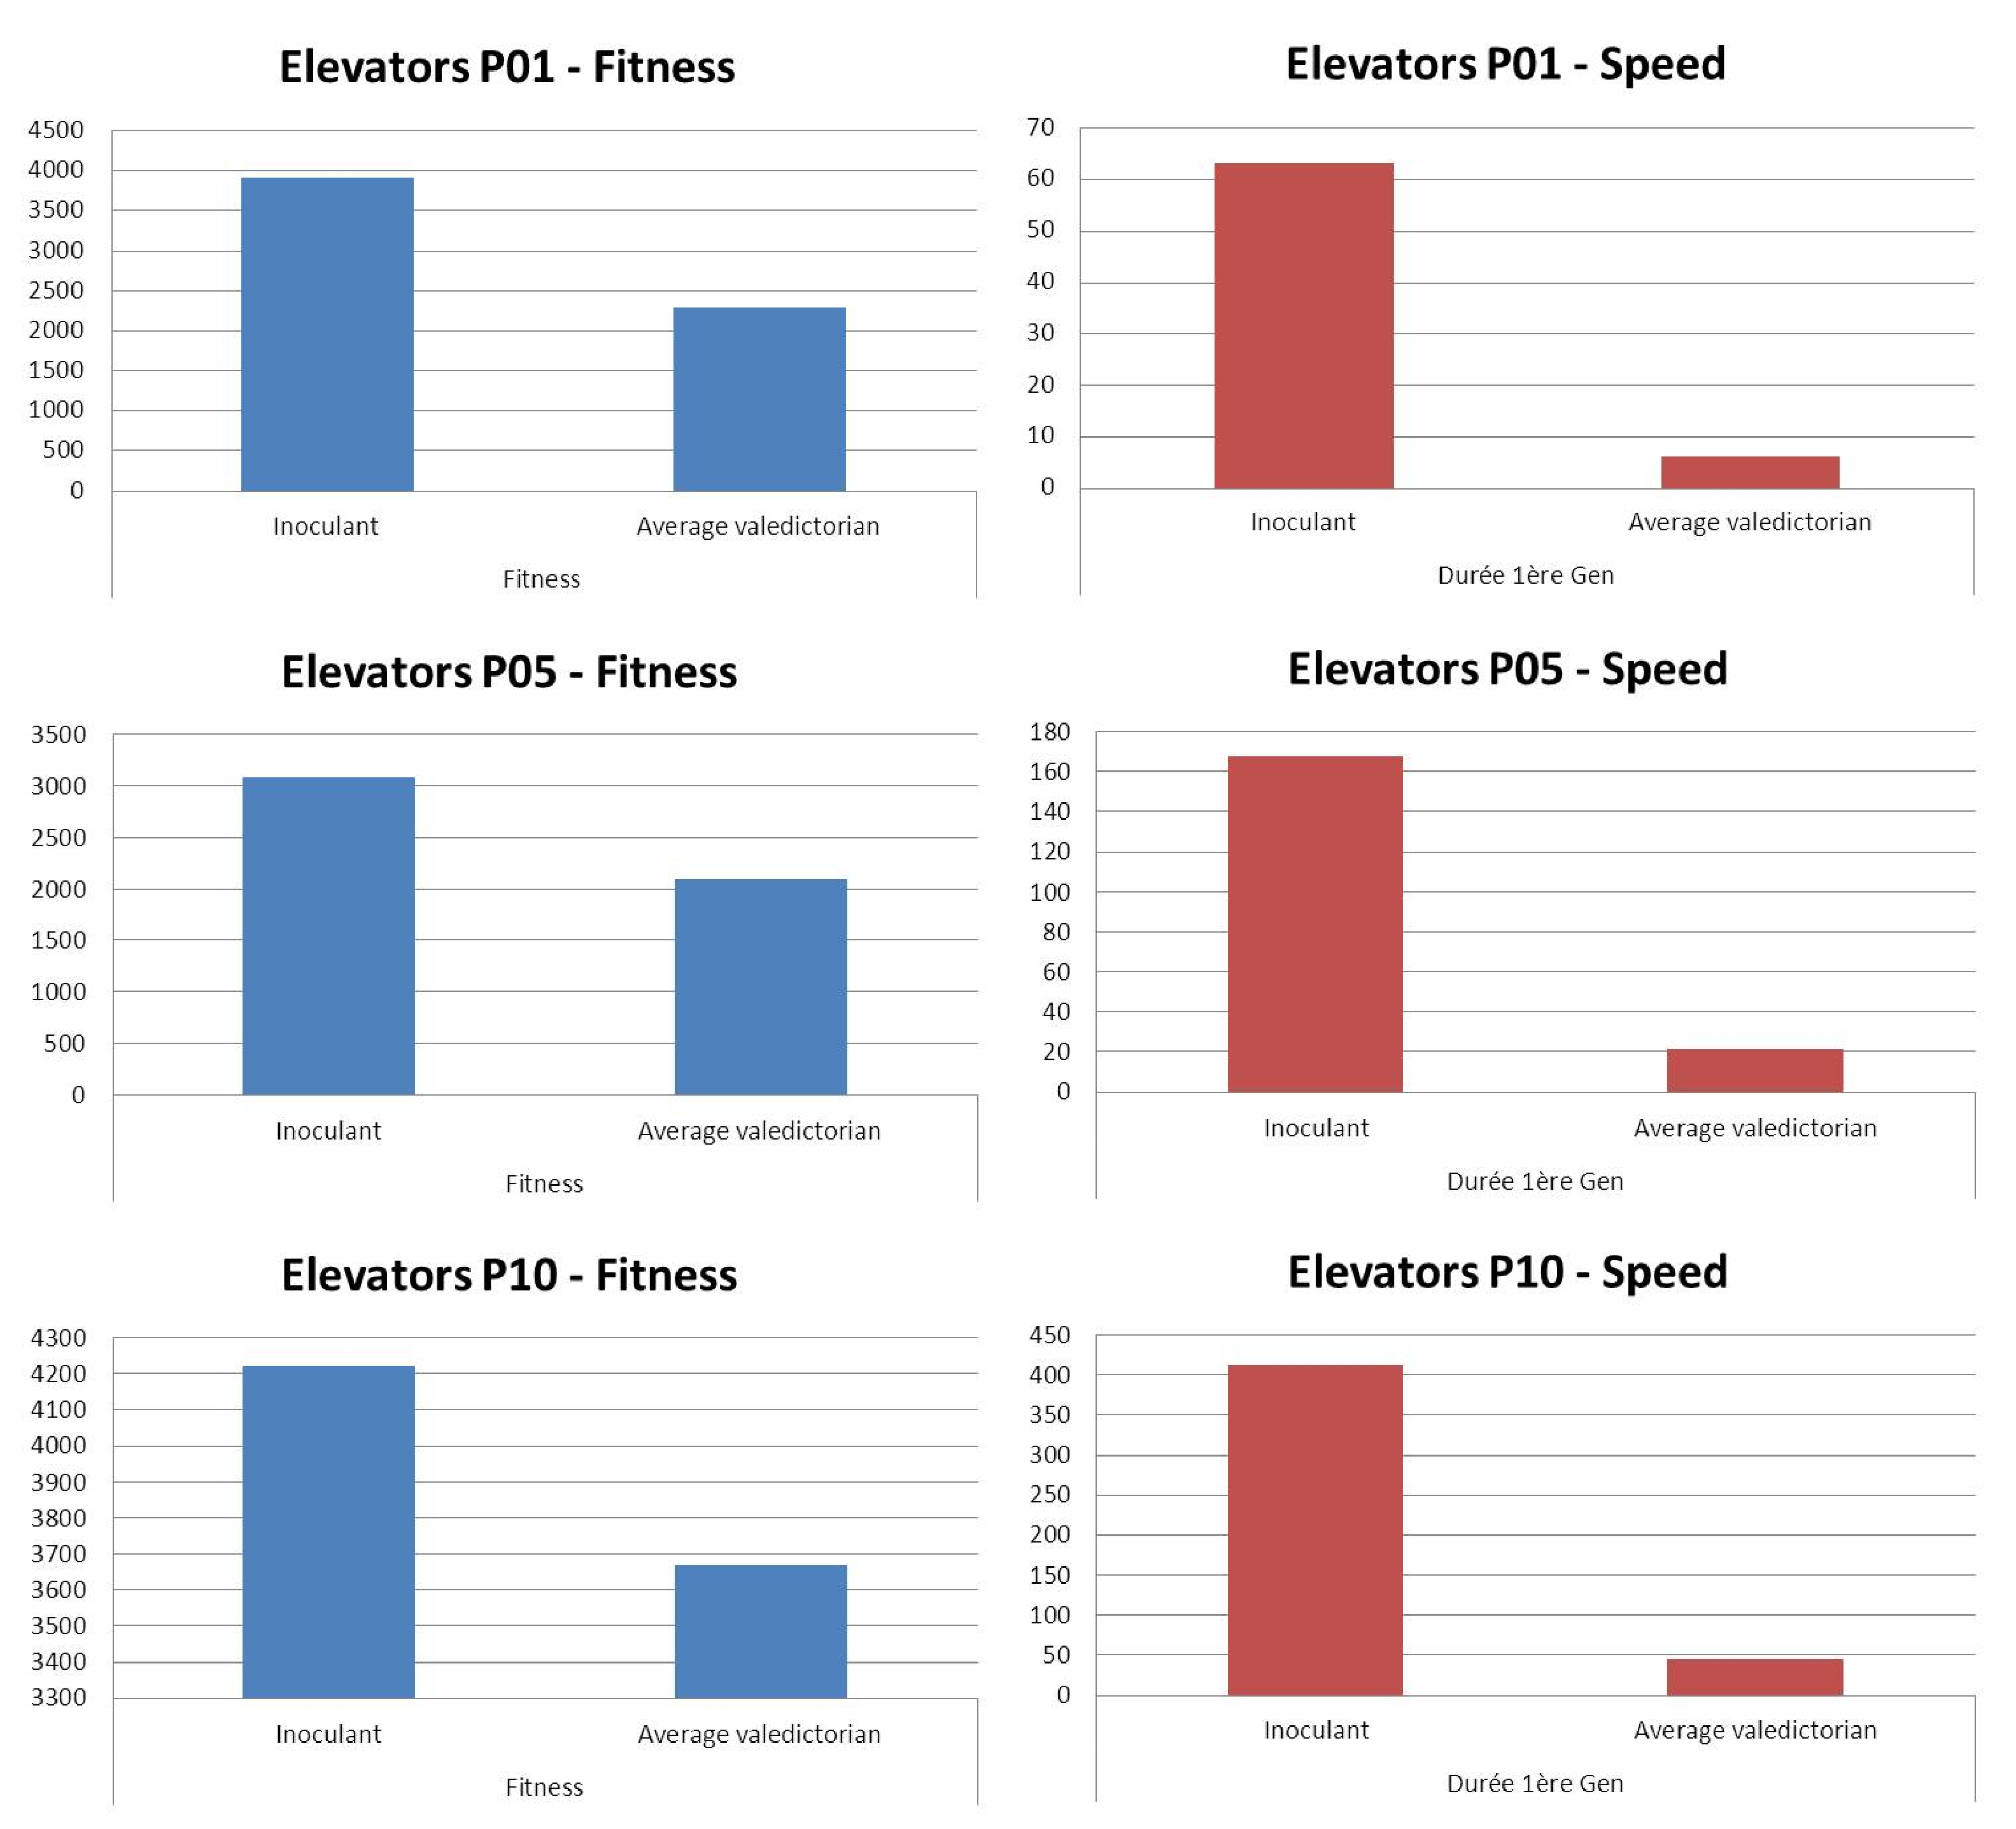
\includegraphics[width=\textwidth]{pics/Elevators.eps}
	\caption{Basic inoculation performance on \ELEVATORS}
	\label{fig:adam_el}
\end{figure}

\begin{figure}
	\centering
		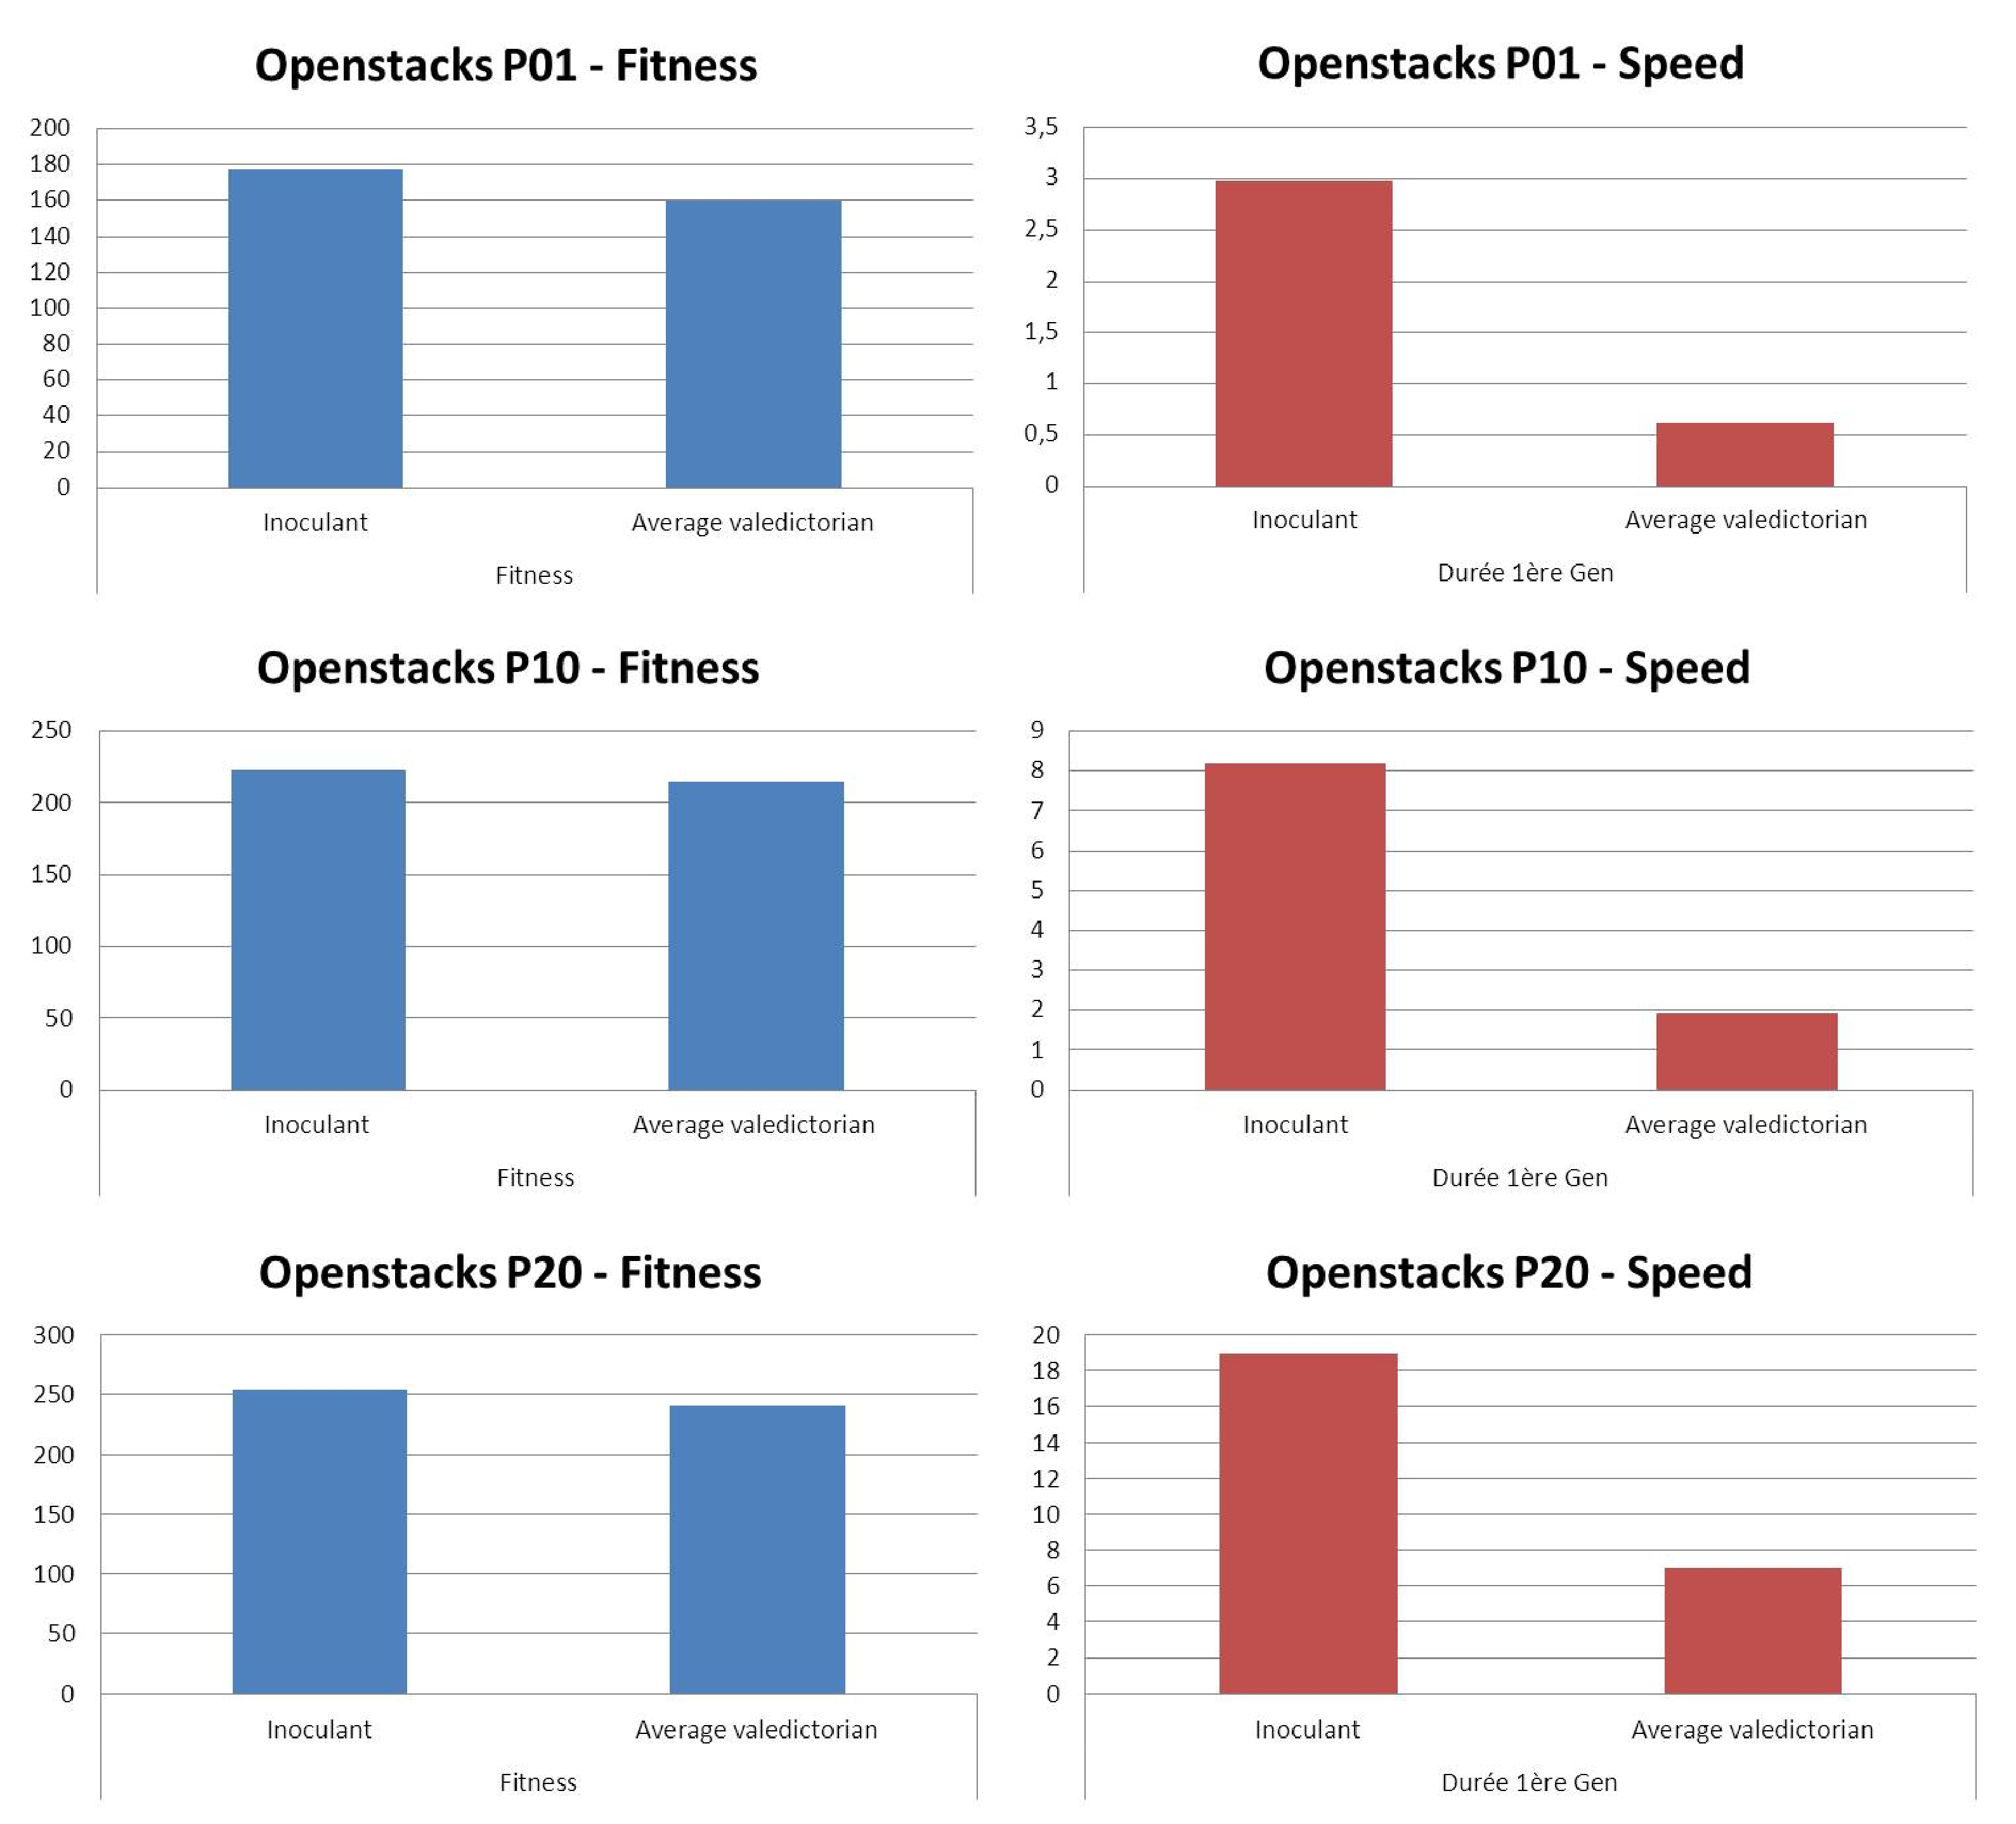
\includegraphics[width=\textwidth]{pics/Openstacks.eps}
	\caption{Basic inoculation performance on \OPENSTACKS}
	\label{fig:adam_open}
\end{figure}


\begin{figure}
	\centering
		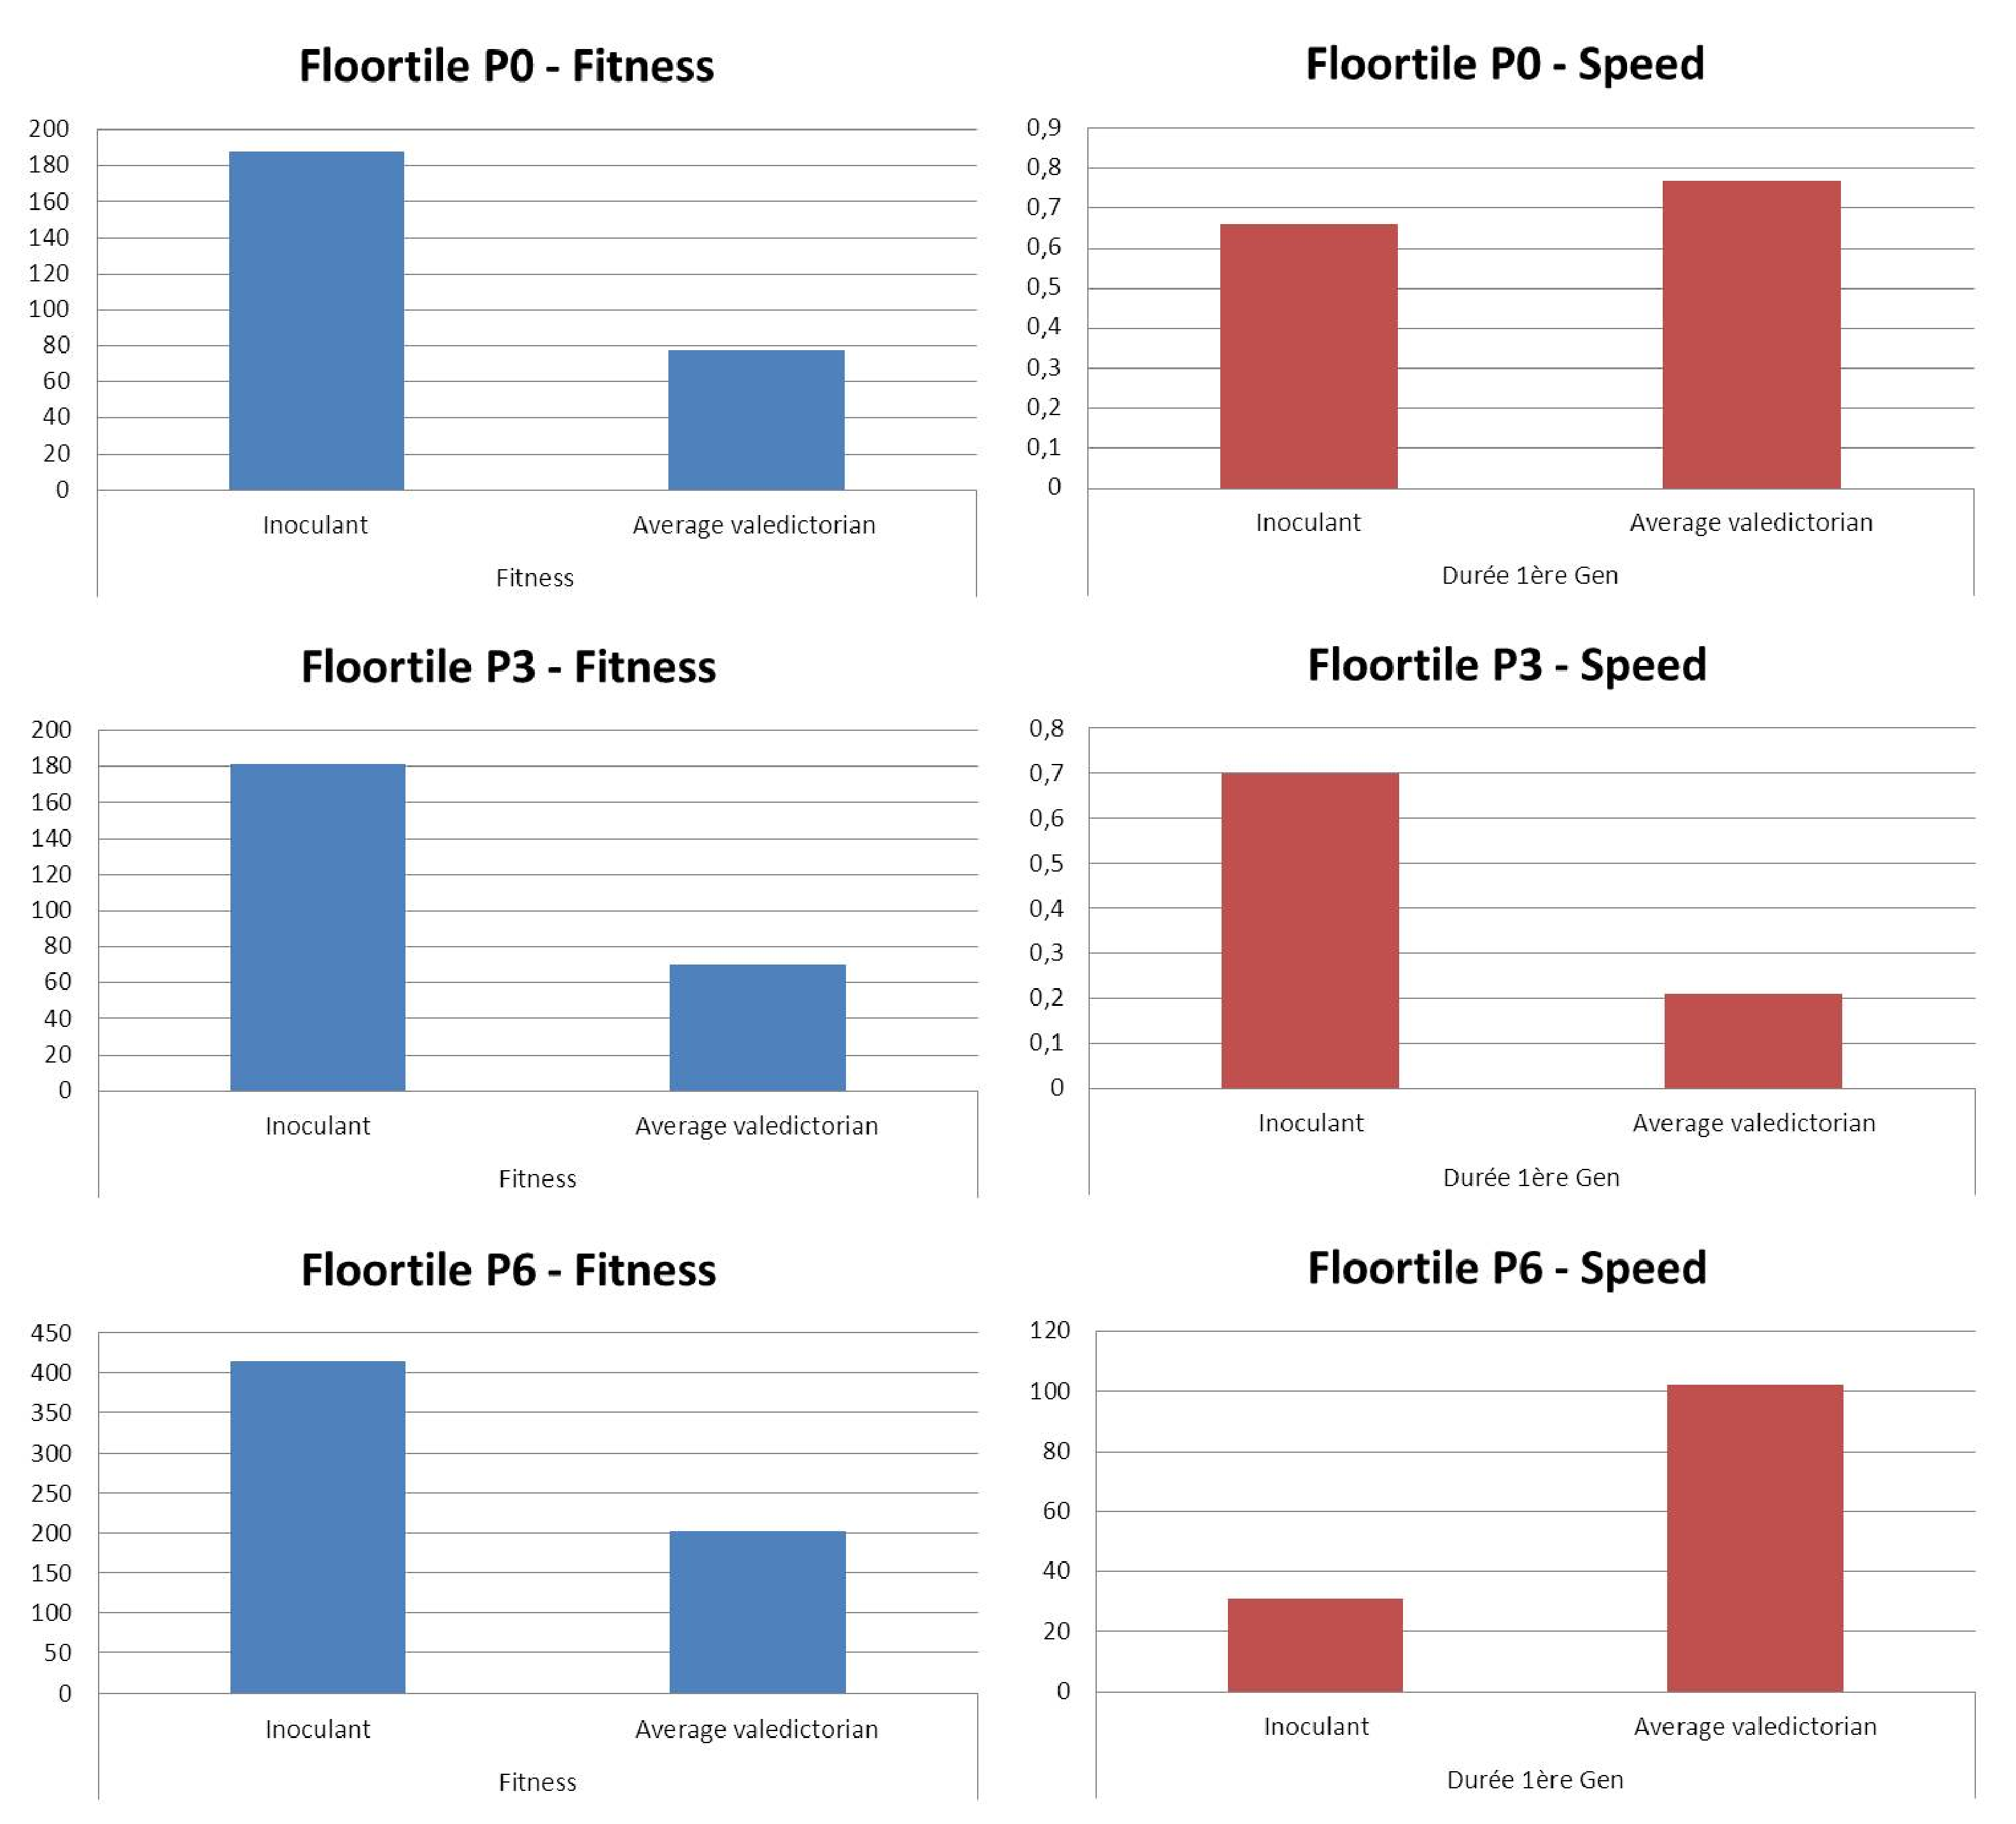
\includegraphics[width=\textwidth]{pics/Floortile.eps}
	\caption{Basic inoculation performance on \FLOORTILE}
	\label{fig:adam_floor}
\end{figure}

\newpage



%\section{Perturbations around Adam}
%Rationale : seeing how Adam can be exploited
%Plots : avg fitness variation with increasing mutation radius (first add adtom then add goal) + proportion of infeasible individuals
%As one can in see in figure \ref{myLabel}, the results are speaking by themselves.

%\begin{figure}
%\begin{figure}[!t]
%\centering
%\includegraphics*[width=10cm,height=10cm]{bmax.png}
%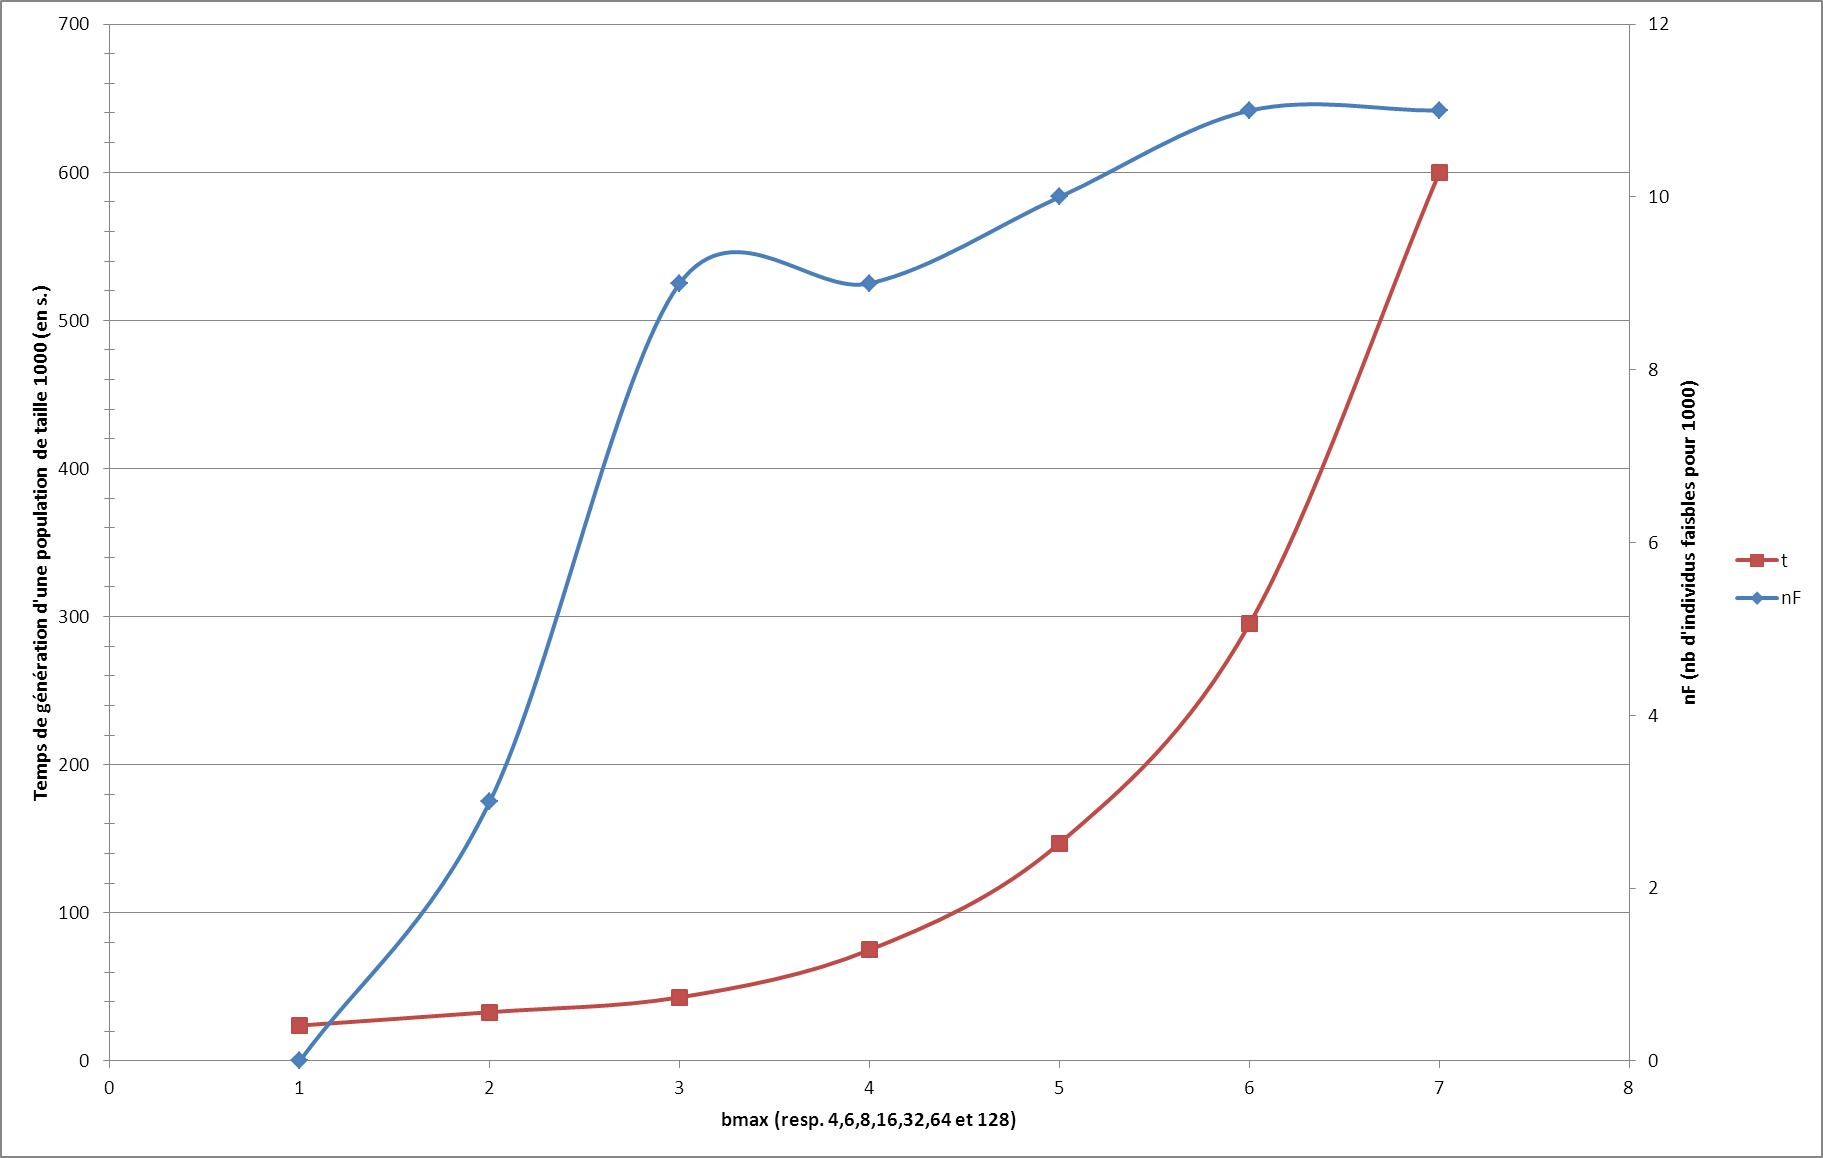
\includegraphics[scale=0.3]{bmax.png}
%\caption{this is the caption}
%\label{myLabel}
%\end{figure}





%\chapter{Population sizing, extra sampling and risk reduction}
\chapter{Inoculation through mass selection}

\section{Motivation and principle}

While observing experimental logs of \dae\ runs performed with or without inoculation, we noticed a number of things in addition to the conclusions reported above. First of all, in many cases, particularly with the \ELEVATORS\ domain, the first challenge our algorithm needs to meet is to find one feasible individual with which it is bound to start the search with our parameter settings. To do so, it follows our loop based bmax estimation procedures which tend to increase bmax exponentially to stand a greater chance to find a way for \YAHSP\ to build a feasible individual around the decompositions. This heuristic works in practice but what we noticed is that it is very costly in terms of speed as runs ending up with high values of bmax tended to be extremely slow. Zooming out it looked like a factor of risk: the run either got a ``lucky'' random seed leading to a feasible individual quickly with a low value of bmax allowing sufficient speed afterward or it got an ``unlucky'' one and got, purely and simply, lost because of unacceptable resulting speed. Another thing we noticed is that benefit of strongly increasing bmax was questionable as many runs, with lucky seeds and therefore low bmax values, could find feasible individuals without difficulty.

From these observations and from those reported above concerning the poor performance of Adam, we derived a new way to initialize, or inoculate our evolutionary algorithm: instead of using \YAHSP\ to find a starting point and instead of increasing bmax to find a first feasible individual, we will simply use additional sampling. In other terms, we will regenerate the initial population randomly with a fixed, low, value of bmax until it contains a feasible individual, which will serve as the inoculant. This very simple scheme should prove useful to reduce the risk of lost runs and increase the average speed at very little cost. The procedure is summarized in algorithm 5 and  the following table:


\begin{algorithm}[h!]
\caption{Inoculation through mass selection}
\label{algoInitMass}
{\small
\begin{algorithmic}[1]
\REQUIRE{$N, b_{max}\-fixed$} \hfill \COMMENT{initialization parameters}

\STATE{$b_{max} =b_{max}\-fixed$}

\STATE{$goodguys \leftarrow 0$}
\WHILE{$((goodguys=0)AND(iter<=maxIter))$} 
\STATE{$goodguys \leftarrow 0$}
\FOR{$i \in [1..N] $}
\STATE{$pop[i] \leftarrow GenerateIndividual(K)$} \hfill \COMMENT{random individuals with K intermediate goals}
\IF{pop[i].isFeasible}
%\STATE{$goodguys++$}
\STATE{$goodguys \leftarrow goodguys+1$}
\ENDIF
\ENDFOR
\ENDWHILE
\end{algorithmic}
}
\end{algorithm}


\begin{center}
\begin{tabular}{|l|l|}
  \hline
  \multicolumn{2}{|c|}{\bf Inoculation through Mass Selection} \\
  \hline
  \emph{Substance provider} & random sampling \\
  \emph{Inoculant builder} & none needed \\
	\emph{Variation scheme} & none \\
	\emph{Composition scheme} & 1 inoculant + random \\
  \hline
\end{tabular}
\end{center}

\section{Experiments}

For all experiments, we use the same parameter settings reported above.

\subsection{Consequences of increasing bmax}

In this first experiment, we formalize our observations that rapidly increasing bmax in search for a first feasible individual is not a viable strategy. To see that, we draw large, random, populations of size 1000 with increasing values of bmax in ranges typical of those observed in runs of \dae\  performed on \ELEVATORS\ P01. As can be seen in figure \ref{fig:bmax}, the number of feasible individuals practically ceases to increase significantly after a bmax value of 8! On the other hand, as one might have suspected, the time it takes to process individuals increases exponentially along with values of bmax as dictated by our estimation procedure. It is therefore clearly not beneficial to increase bmax senselessly: not only does it cost a lot in terms of speed but there is also simply almost no significant benefit to go beyond a certain bmax threshold, here 8.

\begin{figure}
	\centering
		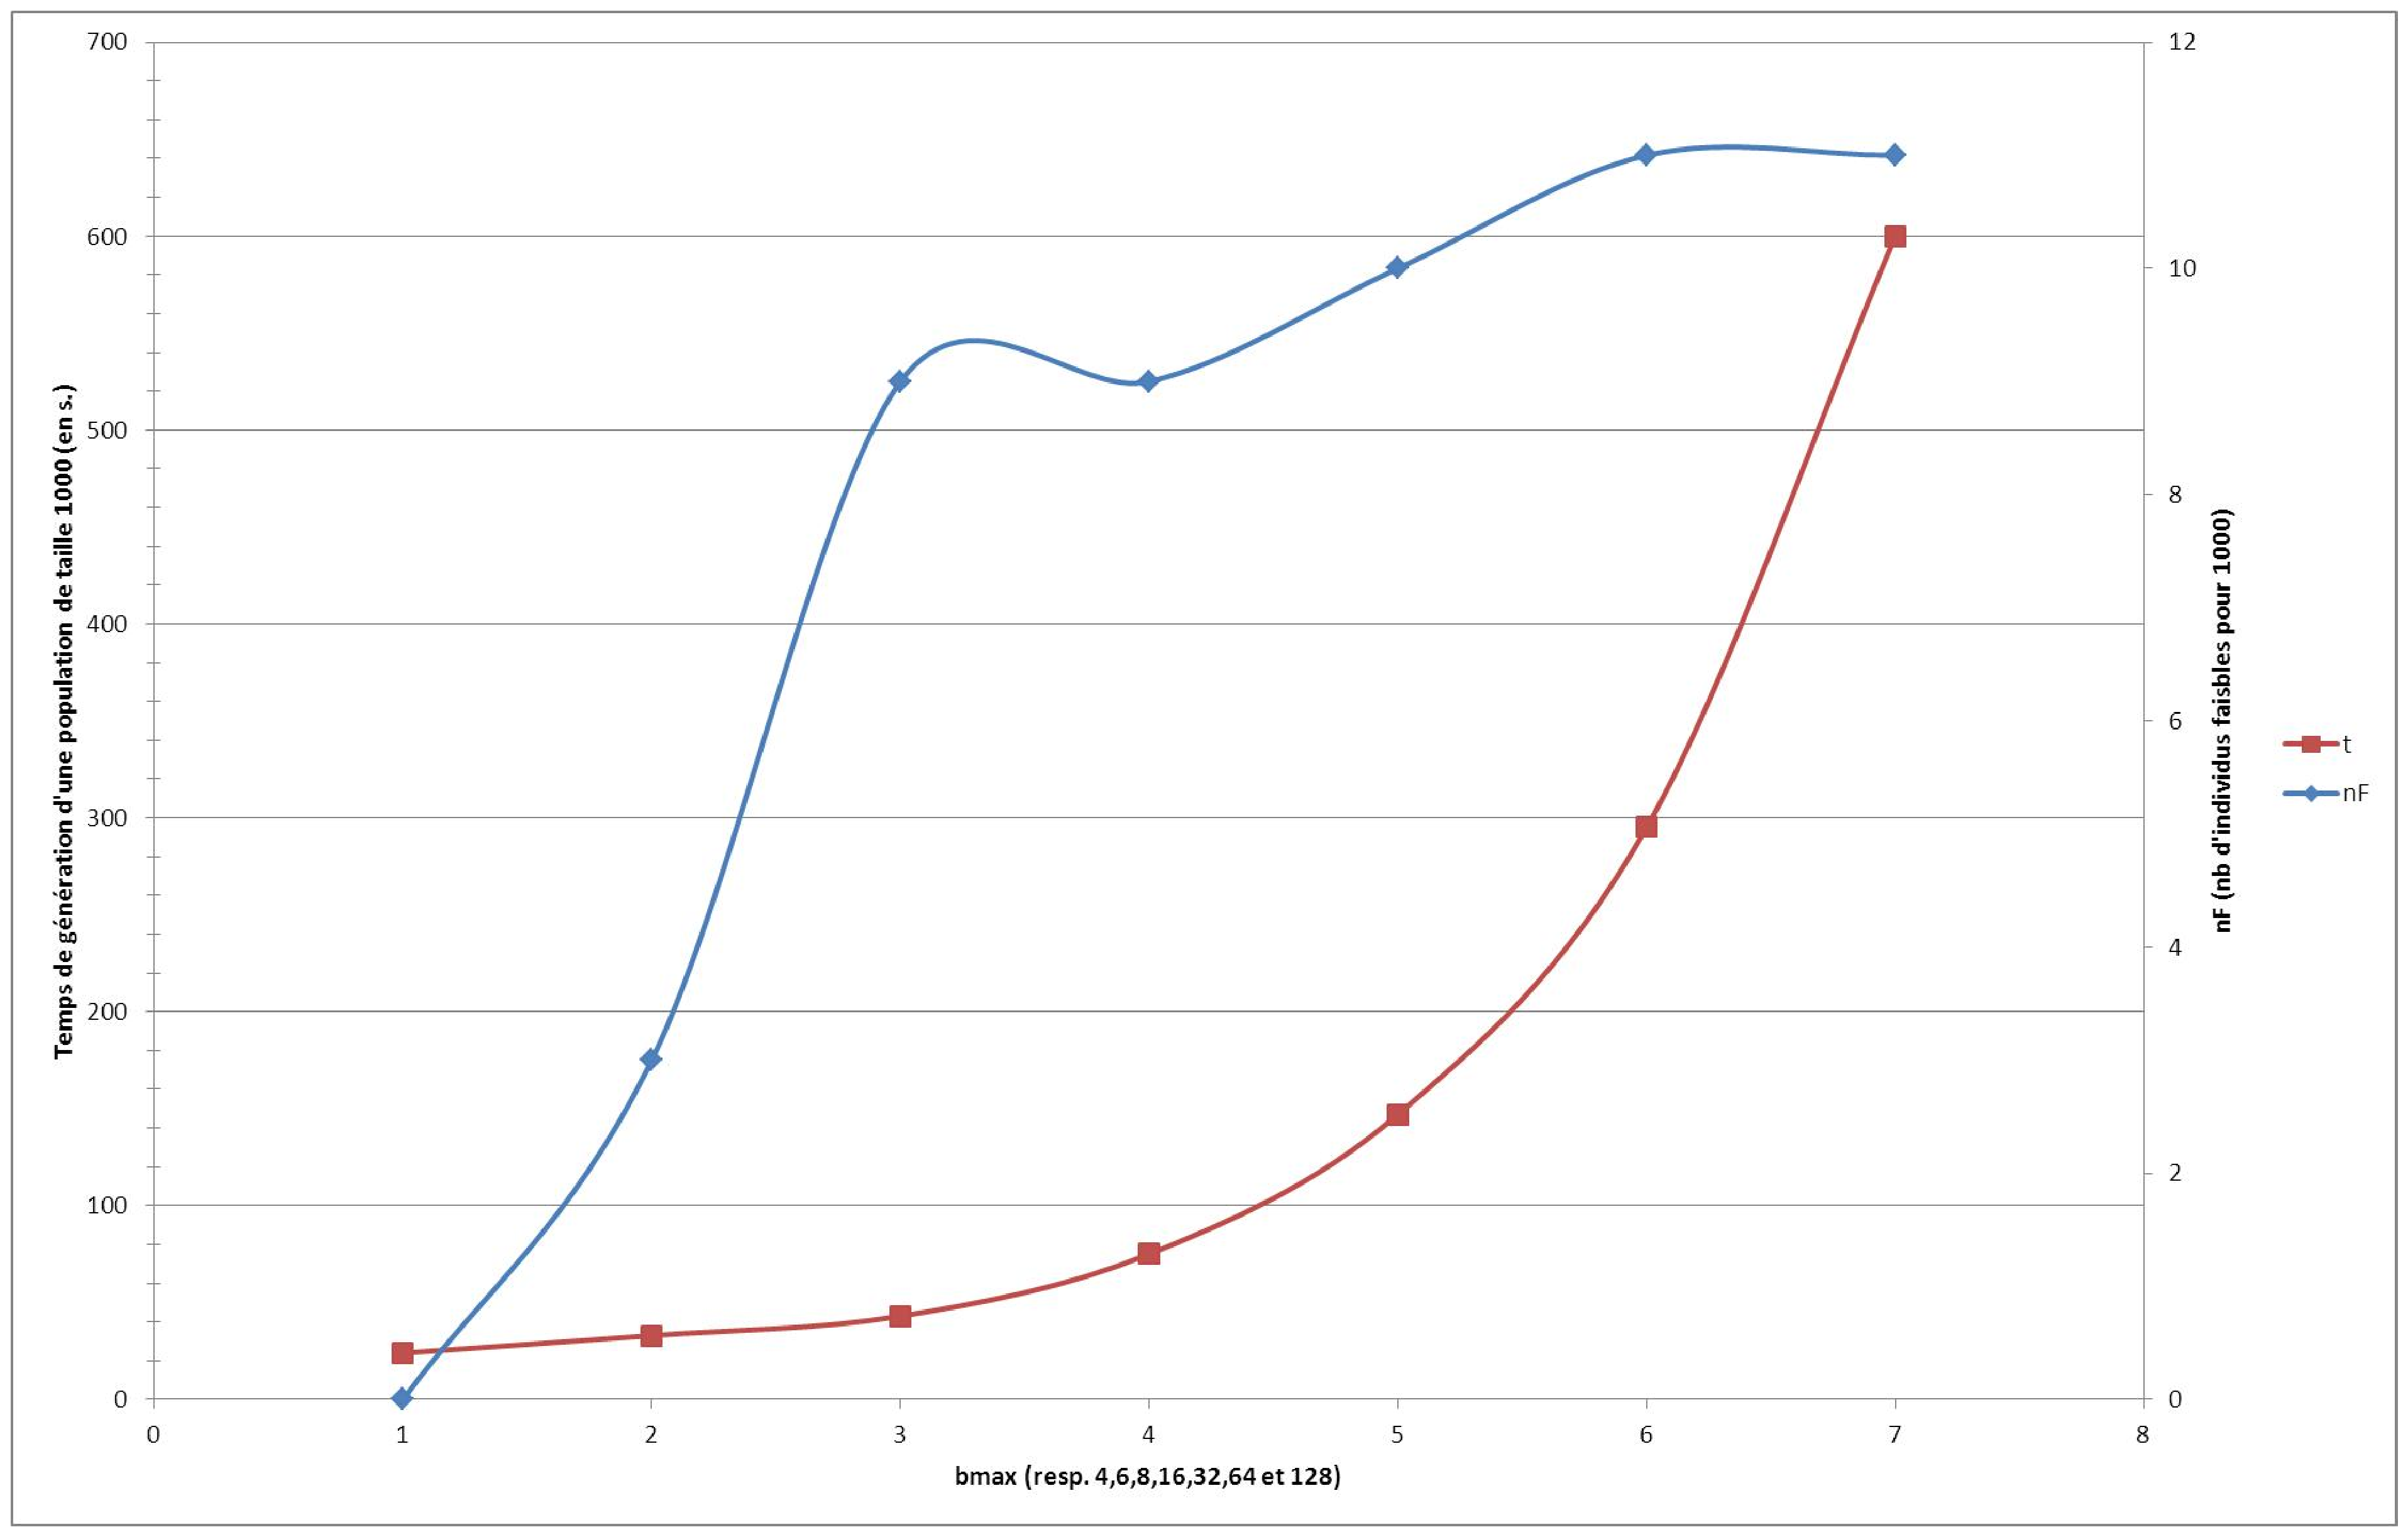
\includegraphics[width=0.9\textwidth]{pics/bmax.eps}
	\caption{The consequences of increasing bmax}
	\label{fig:bmax}
\end{figure}

\subsection{Failure rate}

In this second experiment, we compare the proportions of lost runs between classic initialization and inoculation through mass selection as described above. A successful run is described as run finding a feasible individual to start the search without reaching a bmax value resulting in unreasonable slowness. For this experiment, the threshold for bmax for a run to be considered lost is 32.

As can be seen in figure \ref{fig:failRate}, the failure rate is quite high with the classic procedure as run stands a 25\% to 50\% chance of leading nowhere. Our mass inoculation variant successfully removes that factor of risk on all attempted benchmarks.

\begin{figure}
	\centering
		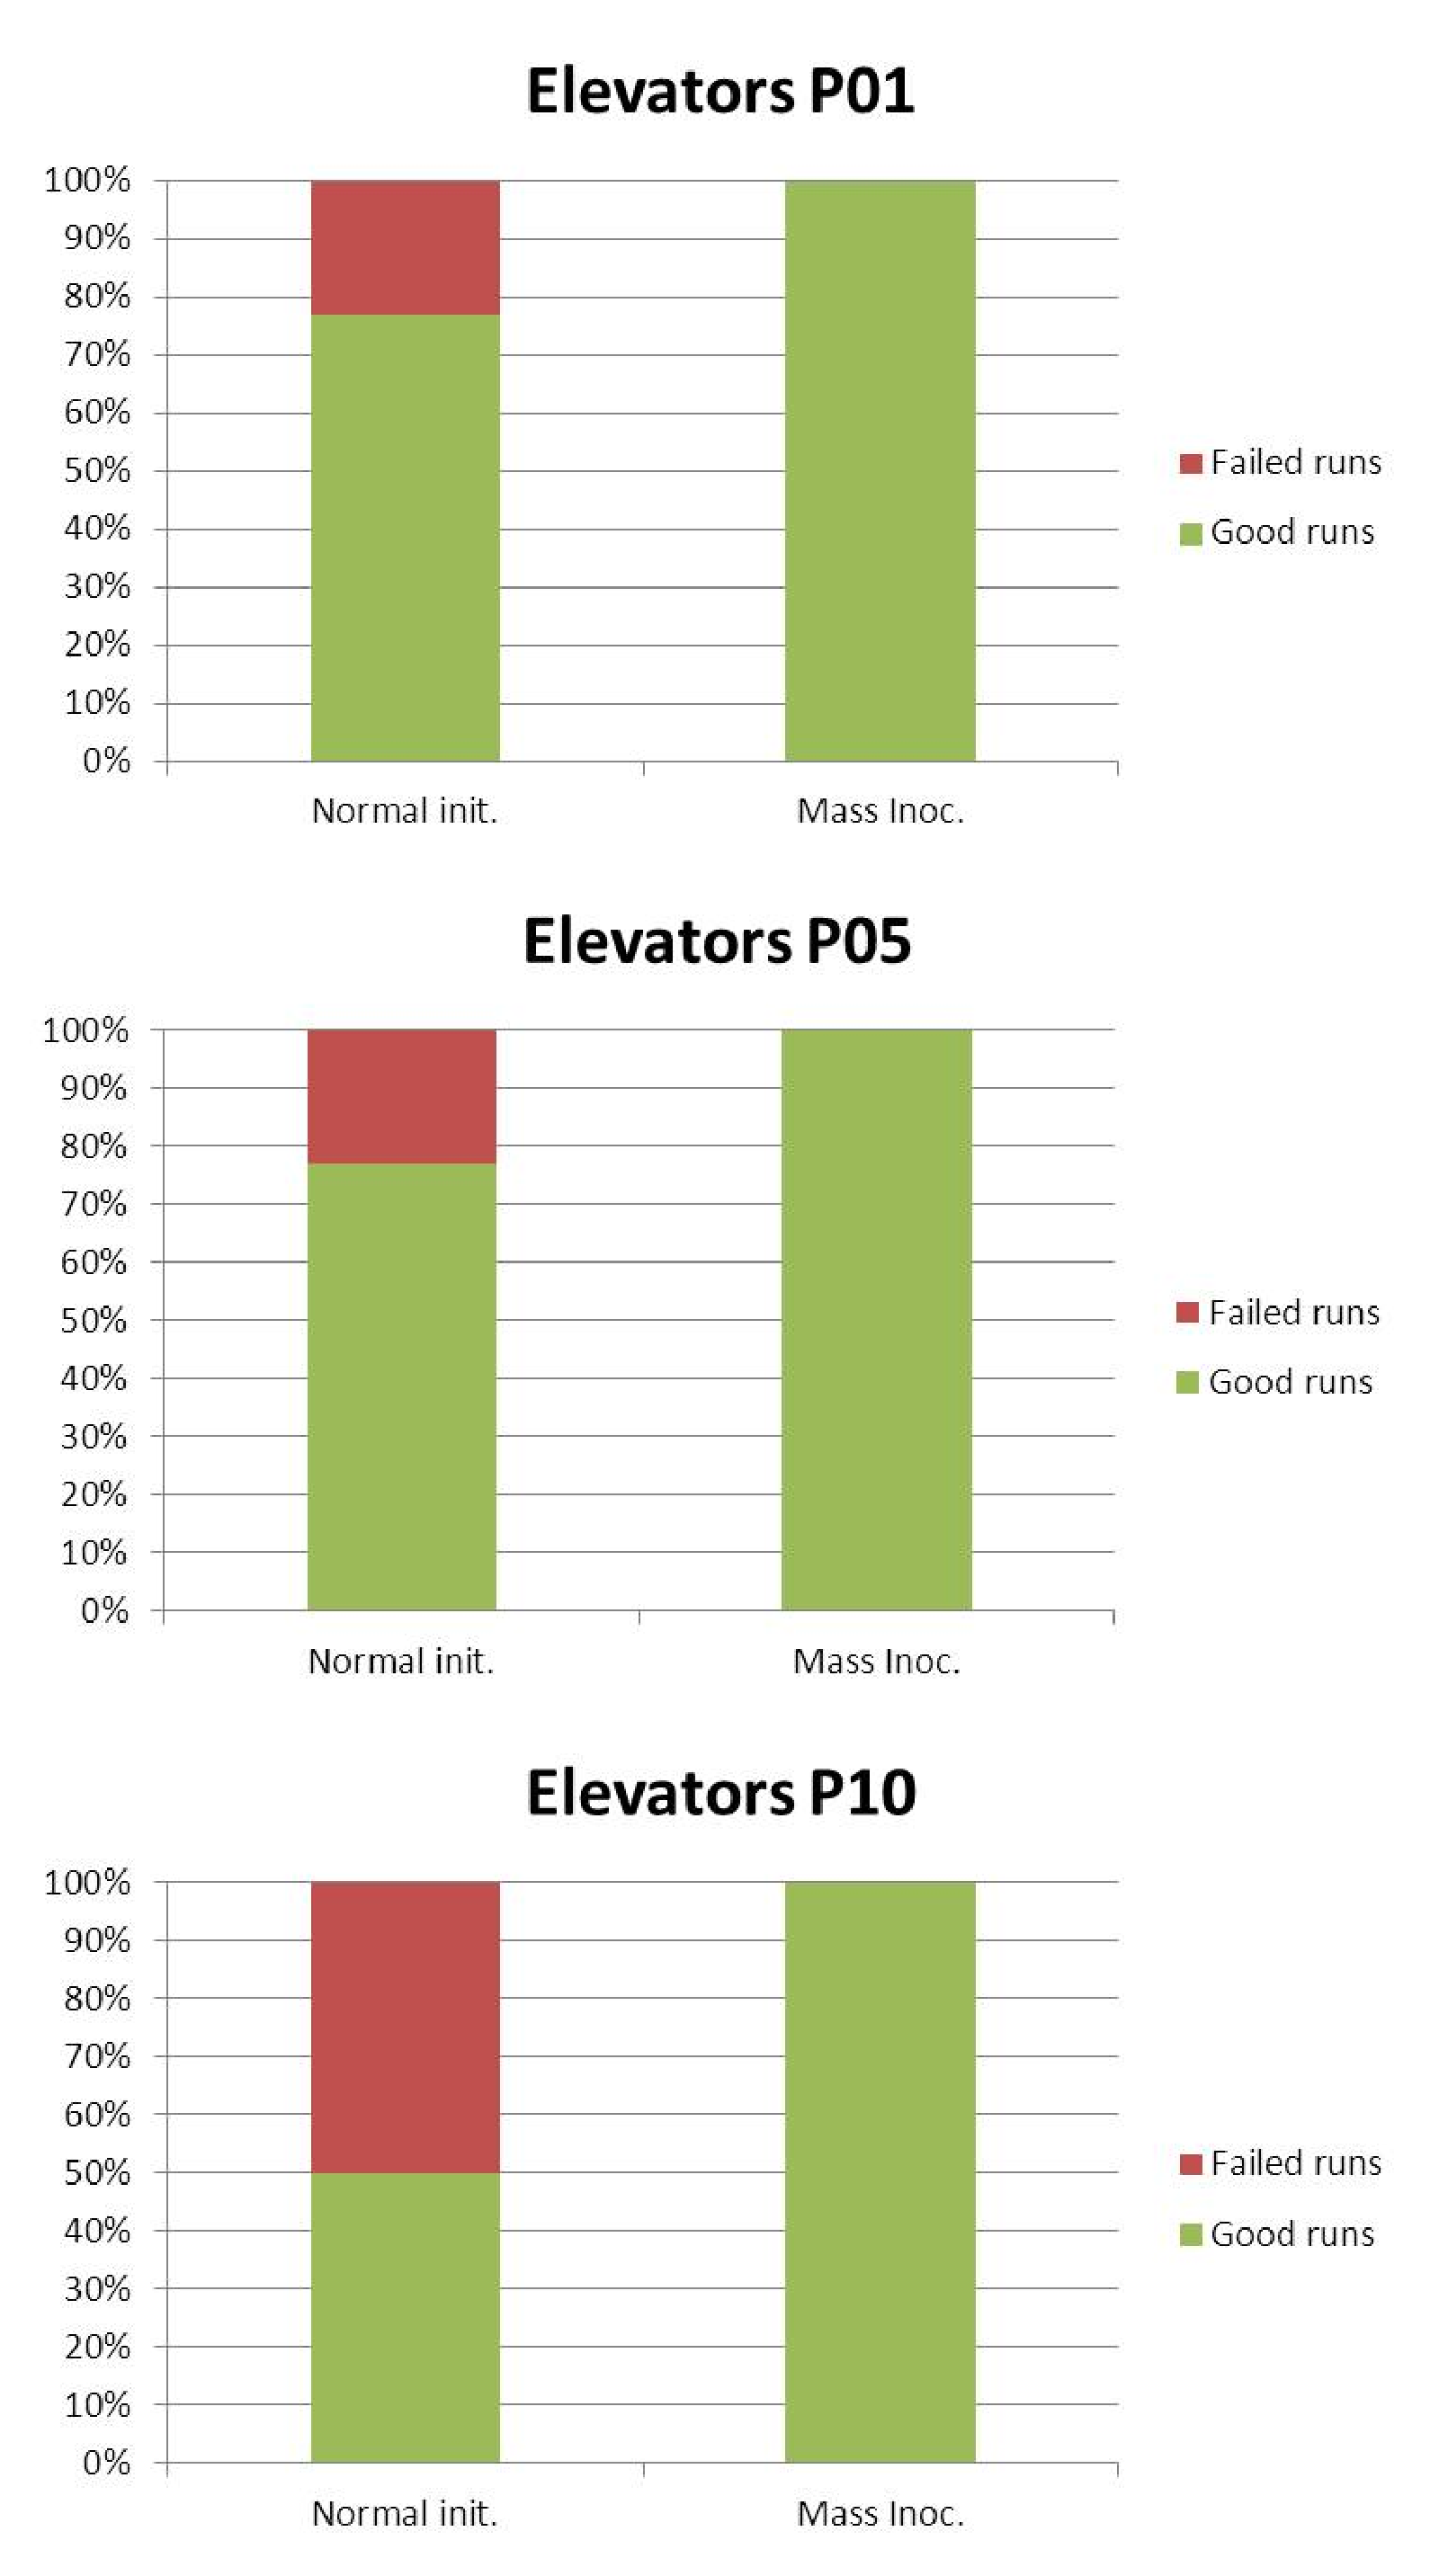
\includegraphics[height=0.8\textheight]{pics/failRate_elevators.eps}
	\caption{Proportion of lost runs on \ELEVATORS}
	\label{fig:failRate}
\end{figure}

\subsection{Start overhead of successful runs}

In the third experiment, we try to look at the cost of this new procedure. Regenerating new random populations and evaluating them is indeed costly as it takes significant time and the start of search is consequently delayed. Figure \ref{fig:overhead} compares the times it takes to reach the first generation in the three cases of interest: classic initialization, classic inoculation and inoculation through mass selection. Although the additional sampling cost is visible with respect to classic initialization, inoculation through mass selection clearly removes the considerable overhead observed with \YAHSP\ based inoculation.

\begin{figure}
	\centering
		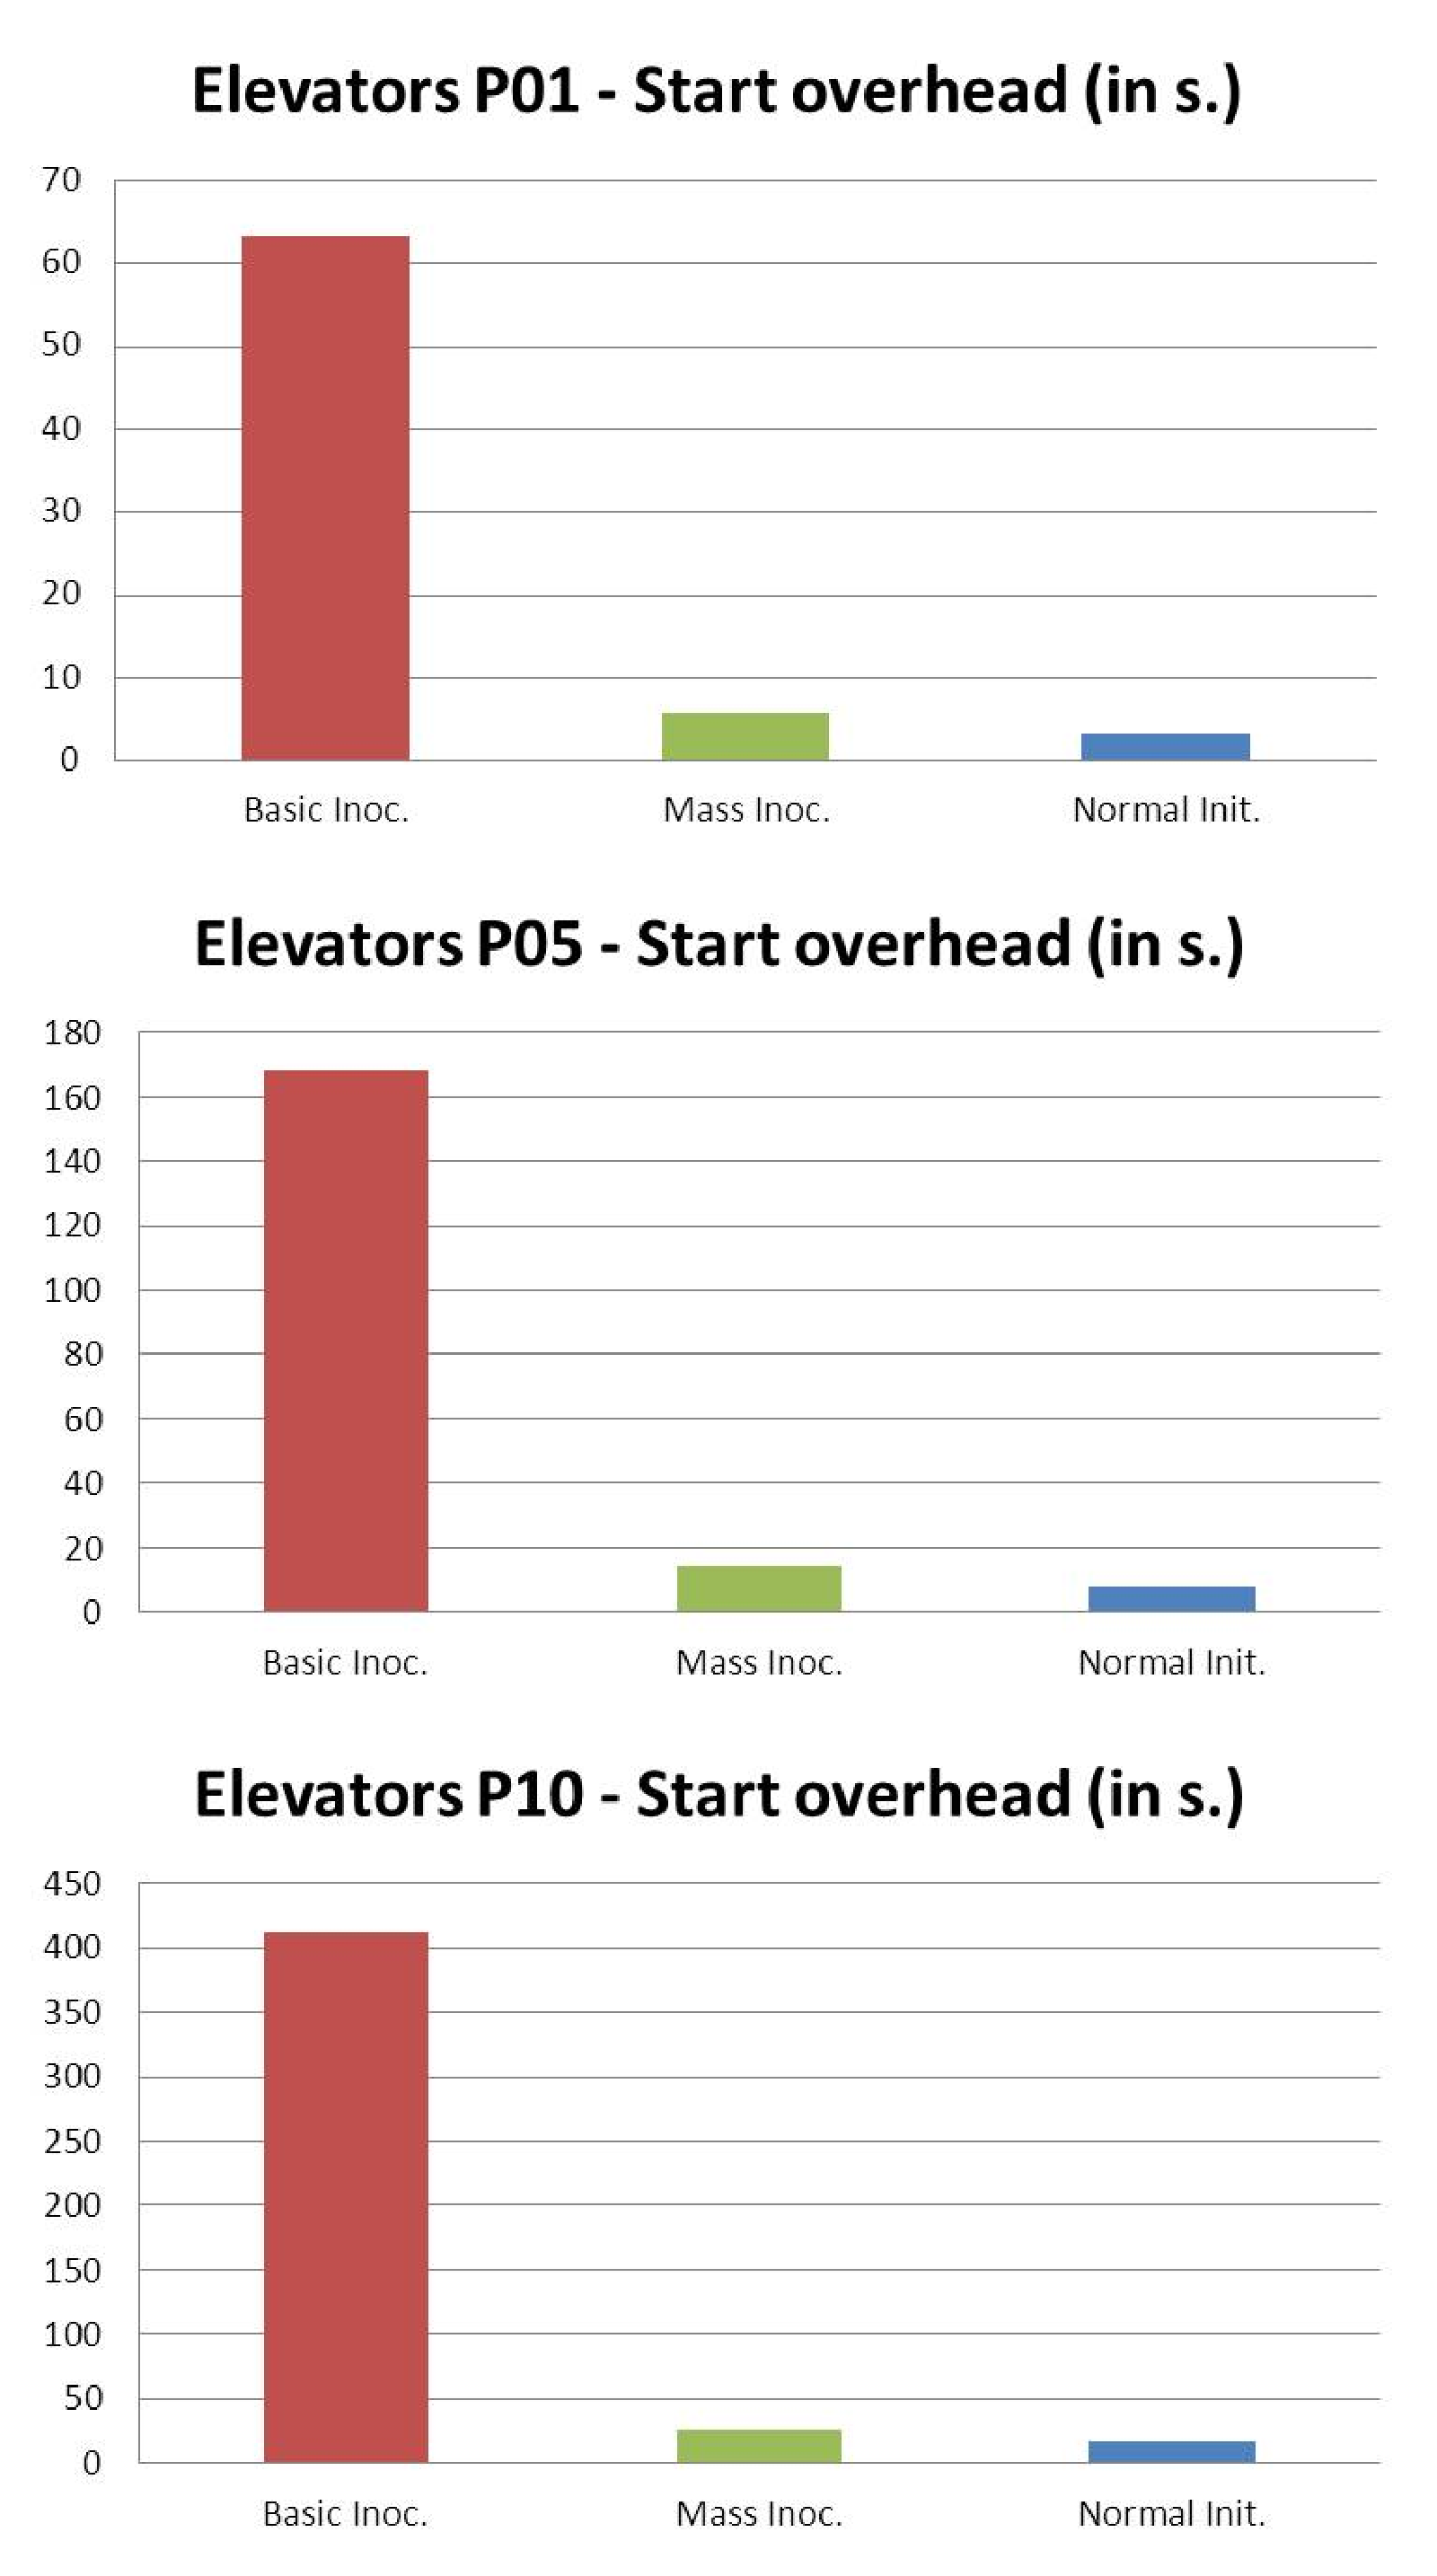
\includegraphics[height=0.8\textheight]{pics/overhead_elevators.eps}
	\caption{Cost of inoculation through mass selection in terms of start overhead}
	\label{fig:overhead}
\end{figure}

\subsection{Average speed over all runs}

In this fourth and last experiment, we observe the benefit of mass inoculation in terms of average speed as opposed to classic initialization. Because it uses a fixed, low value of bmax, mass inoculation has higher resulting average speed than classic initialization which is based on a loop for the estimation of the proper value for bmax which results in a variety of values for bmax over the various runs/seeds, many being, as we saw, pointlessly higher than the manually set value. Of course this calls for a way of automatically coming up with this value but that is left for further work.

\begin{figure}
	\centering
		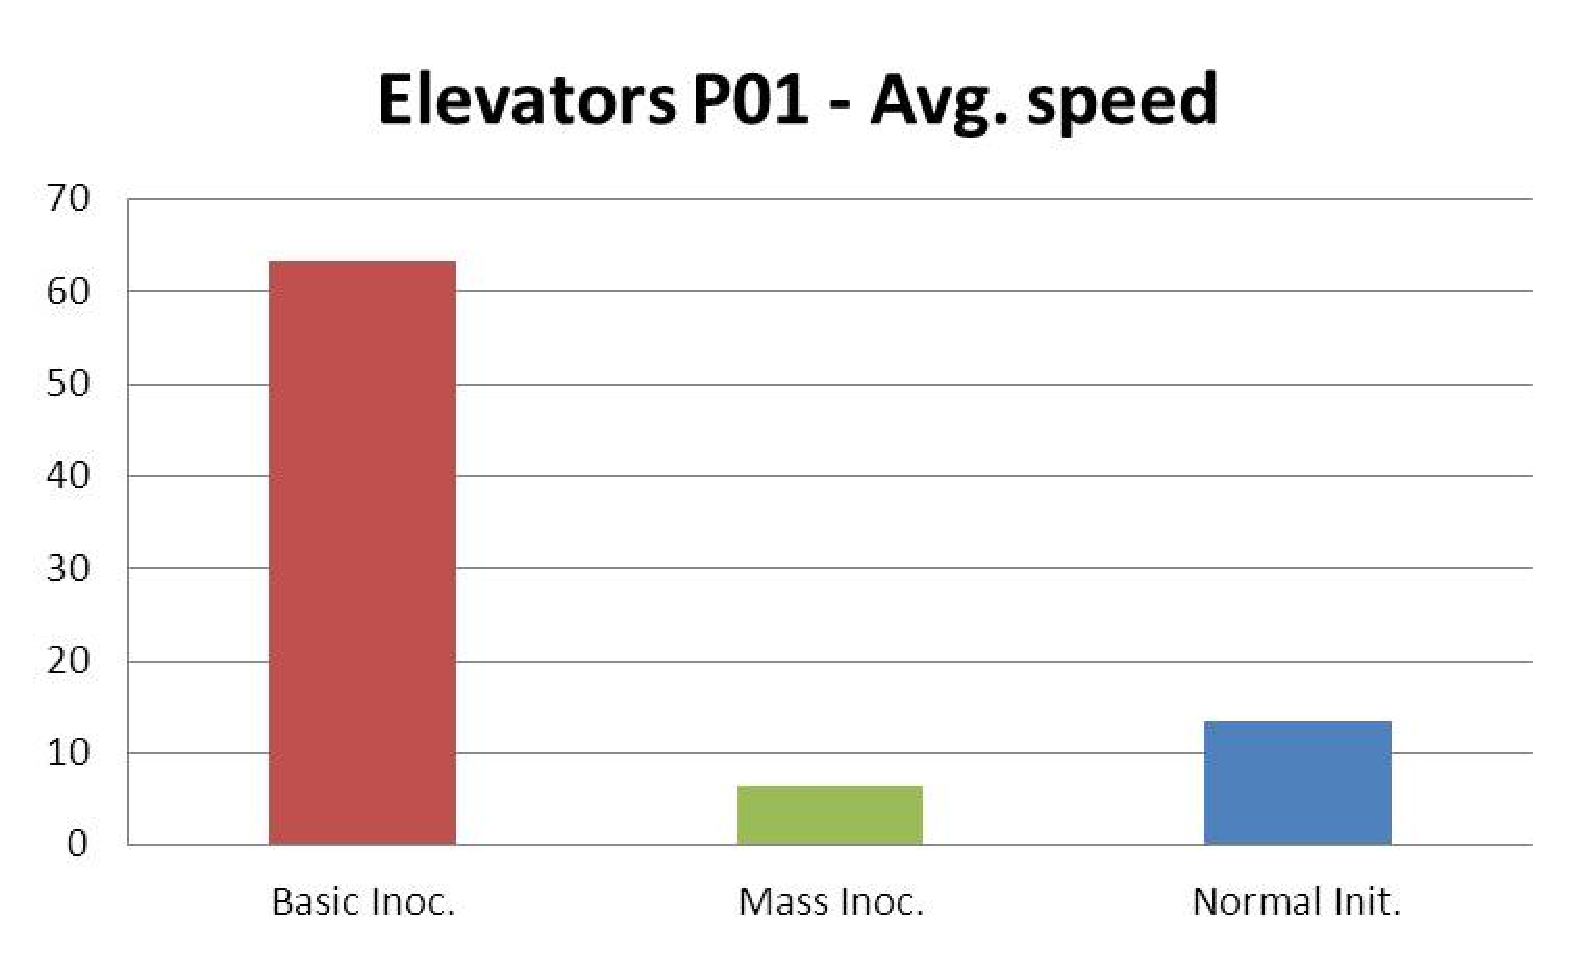
\includegraphics[width=0.6\textwidth]{pics/speed_elevators.eps}
	\caption{Benefit of inoculation through mass selection in terms of average speed}
	\label{fig:bmax2}
\end{figure}

%\section{Smaller populations}
%undersampling vs speed


%\chapter{To Climb Or Not To Climb?}
%\section{Variance in YAHSP}
%\section{Replacement?}


%\chapter{Inoculation with other planners}
%\section{Lama, Popf2, Cpt And Others}
%Inoculation benefit wrt time given to create inoculant

\newpage
\chapter{Conclusion}

Inoculation can be a very good way to improve an evolutionary algorithm's performance in terms of speed, solution quality or robustness. There are many ways to inoculate the population with relevant information and many ways to take advantage of that knowledge. In the context of \dae, we tried two inoculation procedures. The first one, heuristically designed and based on our embedded planner, \YAHSP, performs poorly: the resulting algorithm is slow, risky and produces low quality solutions. Experimental analysis however suggest that further work is required, particularly on the inoculant builder to tweak it and assess the actual benefit of using \YAHSP\ as a substance provider. Observation of experimental results additionally led us to imagine another, very simple, inoculation procedure based on extra sampling which successfully improves our algorithm on a number of benchmarks, in particular by reducing the stochastic risk of runs getting lost. Much further work is however needed to make this improvement robust and significant for all benchmark domains.

\newpage
\newpage
\chapter{References}


\bibliographystyle{plain}
\bibliography{D_5_4}

%\begin{thebibliography}{}
%\bibliographystyle{plain}
%
%\bibitem{AligneSaveant2010}
%Aligne, F.; and Sav\'eant, P.
%\newblock Gestion de crise : optimisation de la mise en {\oe}uvre des plans de secours.
%\newblock In Workshop Interdisciplinaire sur la S{\'e}curit{\'e} Globale ({\em WISG 2010}).
%
%\end{thebibliography}



\end{document}


%\vspace{-0.2cm}
%\begin{algorithm}[h!]
%\caption{evaluate(Ind, planner)}
%\label{algoFitness}
%{\small
%\begin{algorithmic}[1]
%\REQUIRE{$I$, $G$, $b_\text{max}$, $l_\text{max}$}
%\STATE{$k \leftarrow 0 \; ; \; u \leftarrow 0 \; ; \; B \leftarrow 0$}
%\STATE{$i \leftarrow$ I$ \; ; \; g \leftarrow \{\}$}
%\WHILE{$g \neq G$} \label{begin.loop}
%\STATE{$g\leftarrow $ nextGoal(Ind)}
%\STATE{$(sol_k, b_{\text{done}}) \leftarrow \mbox{planner.Solve}(i,g,b_{\text{max}})$} \label{CPT.solve}
%\IF{$sol_k = \bot$} \label{CPT.fail}
%\RETURN {($\bot$, $10\cdot k \cdot \text{\it dist}(i,G) + \text{length(Ind)} - u)$} \label{return.infeasible}
%\ELSIF[\hfill avoid empty plan]{$\text{length}(sol_k) > 0$} \label{useful.states}
%\STATE{$u \leftarrow u+1$} \hfill \COMMENT{useful states counter}
%\STATE{$B \leftarrow B + b_{\text{done}}$} \hfill \COMMENT{total search steps} \label{algo-backtracks}
%\ENDIF
%\STATE{$i \leftarrow$ ExecPlan$(i,sol_k)$}  \hfill \COMMENT{next initial state}\label{global.state}
%\STATE{$k\leftarrow k+1$} \hfill \COMMENT{intermediate goal counter}
%\ENDWHILE \label{end.loop}
%\STATE{$(Sol, Q)\leftarrow \mbox{Compress}((sol_j)_{0 \leq j \leq k})$} \label{CPT.compress}
%\RETURN{$(Sol, Q+\frac{length(Ind)-u+1}{Q} + \frac{B}{l_\text{max} \cdot\, b_\text{max}})$} \label{return.feasible}
%\end{algorithmic}
%}
%\end{algorithm}
%\vspace{-0.2cm}
%
%\vspace{-0.2cm}
%\begin{algorithm}[h!]
%\caption{crossover(Ind$_1$,Ind$_2$)}
%{\small
%\label{algo-crossover}
%\begin{tabbing}
%1: $s_a$ \= $\leftarrow$ \= $\UU($Ind$_1)$ \` // Ind$_1 =(s_i)_{1 \leq i \leq n}$\\
%2: $t_b$ \> $\leftarrow$ \> $\UU($Ind$_2)$ \` // Ind$_2 =(t_i)_{1 \leq i \leq m}$\\
%3: {\bf if} $\Delta(t_b) > \Delta(s_a)$ \= {\bf then} \= {\bf return} \= $(s_1,\ldots,s_a,t_b,\ldots,t_m)$\\
%4: \> {\bf else} \> {\bf return} \> $(t_1,\ldots,t_b,s_a,\ldots,s_n)$
%\end{tabbing}
%}
%\vspace{-0.2cm}
%\end{algorithm}
%\vspace{-0.3cm}
%
%\vspace{-0.2cm}
%\begin{algorithm}[h!]
%\caption{addGoal(Ind)}
%\label{algo-addGoal}
%{\small
%\begin{algorithmic}[1]
%\REQUIRE{$r$} \hfill \COMMENT{neighborhood radius}
%\STATE{$j \leftarrow \UU$([1, min(length(Ind),lastReached(Ind))])}
%\STATE{$s\leftarrow \{\}$} \hfill \COMMENT{insert $s$ between $s_j$ and $s_{j+1}$}
%\STATE{$t \leftarrow \UU(\{t \in T\;|\; \Delta(s_j) < t \leq \Delta(s_{j+1}) \})$} %\hfill \COMMENT{$\Delta(s_j) < t \leq \Delta(s_{j+1})$}
%\STATE{$A_t \leftarrow \{a \in A \;|\; T(a)\in \text{neighbourhood}(t,r) \} $} 
%\STATE{$A_m\leftarrow \{\}$ } \hfill \COMMENT{set of non pairwise mutex atoms}
%\WHILE{$A_t\neq \{\}$}
%\STATE{$a \leftarrow \UU(A_t)$}
%\STATE{$A_m\leftarrow A_m\cup \{a\}$ }
%\STATE{$A_t \leftarrow A_t \setminus (\{a\}\cup M(a))$}
%\ENDWHILE
%\STATE{$N \leftarrow \UU([1,\#A_m])$} \hfill \COMMENT{goal length}
%\REPEAT 
%\STATE{$a \leftarrow \UU(A_m)$} \hfill \COMMENT{choose uniformly an atom in $A_m$}
%\STATE{$s \leftarrow s \cup \{a\}$} \hfill \COMMENT{add to $s$}
%\STATE{$A_m\leftarrow A_m \setminus \{a\}$}\hfill \COMMENT{remove from $A_m$ }
%\UNTIL{$\#s = N$}
%\STATE{insert(Ind, $s$, $j$)} \hfill \COMMENT{insert $s$ after goal j}
%\RETURN{Ind}
%\end{algorithmic}
%}
%\end{algorithm}
%\vspace{-0.3cm}
%
%\vspace{-0.2cm}
%\begin{algorithm}[h!]
%\caption{addAtom(Ind)}
%\label{algo-modifstateadd}
%{\small
%\begin{algorithmic}[1]
%\REQUIRE {$p_c, p_a$} \hfill \COMMENT{relative probabilities to change or add an atom}
%\FORALL{$k \in$ [1,min(length(\text{Ind}),lastReached(\text{Ind})+1)]}
%\IF[\hfill atom change]{$\UU([0,1]) < \frac{p_c}{\text{length(Ind)}}$}
%\STATE{$a \leftarrow \UU(\text{Ind}[k])$}
%\STATE{$b \leftarrow \UU(\{b \in M(a)\;|\;T(b)=\Delta(\text{Ind}[k]) \land \nexists c  \in \quad~\hskip 0.8cm (\text{Ind}[k] \setminus \{a\}), b \in M(c)\})$}
%\STATE{$\text{Ind}[k] \leftarrow (\text{Ind}[k] \setminus \{a\}) \cup \{b\}$}
%\ENDIF
%\IF[\hfill atom addition]{$\UU([0,1]) < p_a$}
%\STATE{$a \leftarrow \UU(\{b \in A\;|\; T(b) = \Delta(\text{Ind}[k]) \land \nexists c \in \quad~\hskip 1cm \text{Ind}[k], b \in M(c)\})$}
%\STATE{$\text{Ind}[k] \leftarrow \text{Ind}[k] \cup \{a\}$}
%\ENDIF
%\ENDFOR
%\RETURN{Ind}
%\end{algorithmic}
%}
%\end{algorithm}
%\vspace{-0.4cm}
%
%
%\vspace{-0.2cm}
%\vspace{-0.2cm}
%
%\begin{algorithm}[tb!]
%\caption{DAEX({\scriptsize popSize, OffSpringSize, MaxGen, MaxChgt,} {\small p$_\text{cross}$, p$_\text{mut}$, w$_\text{addGoal}$, w$_\text{delGoal}$, w$_\text{addAtom}$, w$_\text{delAtom}$, b$_\text{max}$, l$_\text{max}$, $r, p_c, p_a$})}
% {\scriptsize // Main loop: $h=h^1$ popSize=100, OffSpringSize = 700}}
%\label{algoMain}
%{\small
%\begin{algorithmic}[1]
%\REQUIRE{planner, $h$}\hfill \COMMENT{embedded planner and heuristic function}
%\FORALL{$a \in A$}
%\STATE{$T(a) \leftarrow h(a)$} \hfill \COMMENT{compute earliest start time}
%\ENDFOR
%\STATE{$T \leftarrow \{T(a) \neq 0\;|\;a \in A\}$} \hfill \COMMENT{candidate start times set}
%\STATE{pop $\leftarrow$ \{\}} \hfill \COMMENT{start building the population}
%\REPEAT
%\STATE{pop $\leftarrow$ pop $\cup$ \{GenerateIndividual($\UU([1,\#T])\}$)} \label{init.sequence}
%\UNTIL{$\#$pop = popSize}
%\REPEAT \label{main.loop}
%\STATE{offspring $\leftarrow$ \{\}}
%\REPEAT
%\STATE{Ind$_1$ $\leftarrow$ $\UU$(pop)}
%\IF{$\UU([0,1])$ $<$ p$_\text{cross}$}
%\STATE{Ind$_2$ $\leftarrow$ $\UU$(pop)}
%\STATE{Newind $\leftarrow$ crossover(Ind$_1$,Ind$_2$)}
%\ELSE
%\STATE{Newind $\leftarrow$ Ind$_1$}
%\ENDIF
%\IF{$\UU([0,1])$ $<$ p$_\text{mut}$}
%\STATE{$f \leftarrow$ $\UU_\text{weighted}$({\scriptsize addGoal, addAtom, delGoal, delAtom, w$_\text{addGoal}$, w$_\text{delGoal}$, w$_\text{addAtom}$, w$_\text{delAtom}$})}
%\STATE{Newind $\leftarrow$ APPLY($f$, Newind)}
%\ENDIF
%\STATE{offspring $\leftarrow$ offspring $\cup$ \{Newind\}}
%\UNTIL{$\#$offspring = OffSpringSize}
%\FORALL{Ind $\in$ pop $\cup$ offspring}
%\STATE{Evaluate(Ind, planner)}
%\ENDFOR
%\STATE{pop $\leftarrow$ SurvivalSelection(pop $\cup$ offspring)}\label{main.survival}
%\UNTIL{$\#$gen $>$ MaxGen OR noImprovementSince(MaxChgt)}
%\RETURN{Evaluate(pop.BestIndividual, planner).Sol}
%\end{algorithmic}
%}
%\end{algorithm}
